\section{Introduction}
The spread of COVID-19 has elevated the importance of epidemiological
models as a means to forecast both near- and long-term spread. 
In the United States, the Institute for Health Metrics and Evaluation (IHME)
model has emerged as a key influencer of state- and national-level
policy \citep{covid2020forecasting}.  
The IHME model includes a detailed characterization
of the variation in
hospital bed capacity, ICU beds, and ventilators between and within
states. Predicting the projected strains on underlying
health resources is critical to supporting planning efforts.
However such projections require
an epidemic `forecast'.  Early versions of IHME's epidemic forecast
differed from conventional
epidemic models in a significant way -- IHME assumed
that the cumulative deaths in the COVID-19 epidemic 
followed a symmetric, Gaussian-like trajectory. 
For example, the 
IHME model predicted that if the peak is 2 weeks away then in 4 weeks
cases will return to the level of the present, and continue
to diminish rapidly.  But, epidemics need not have one symmetric peak -- 
the archaic Farr's Law of Epidemics notwithstanding
(see~\citep{bregman1990farr} for a cautionary tale of using
Farr's law as applied to the HIV epidemic). 
\begin{figure*}[t!]
\begin{center}
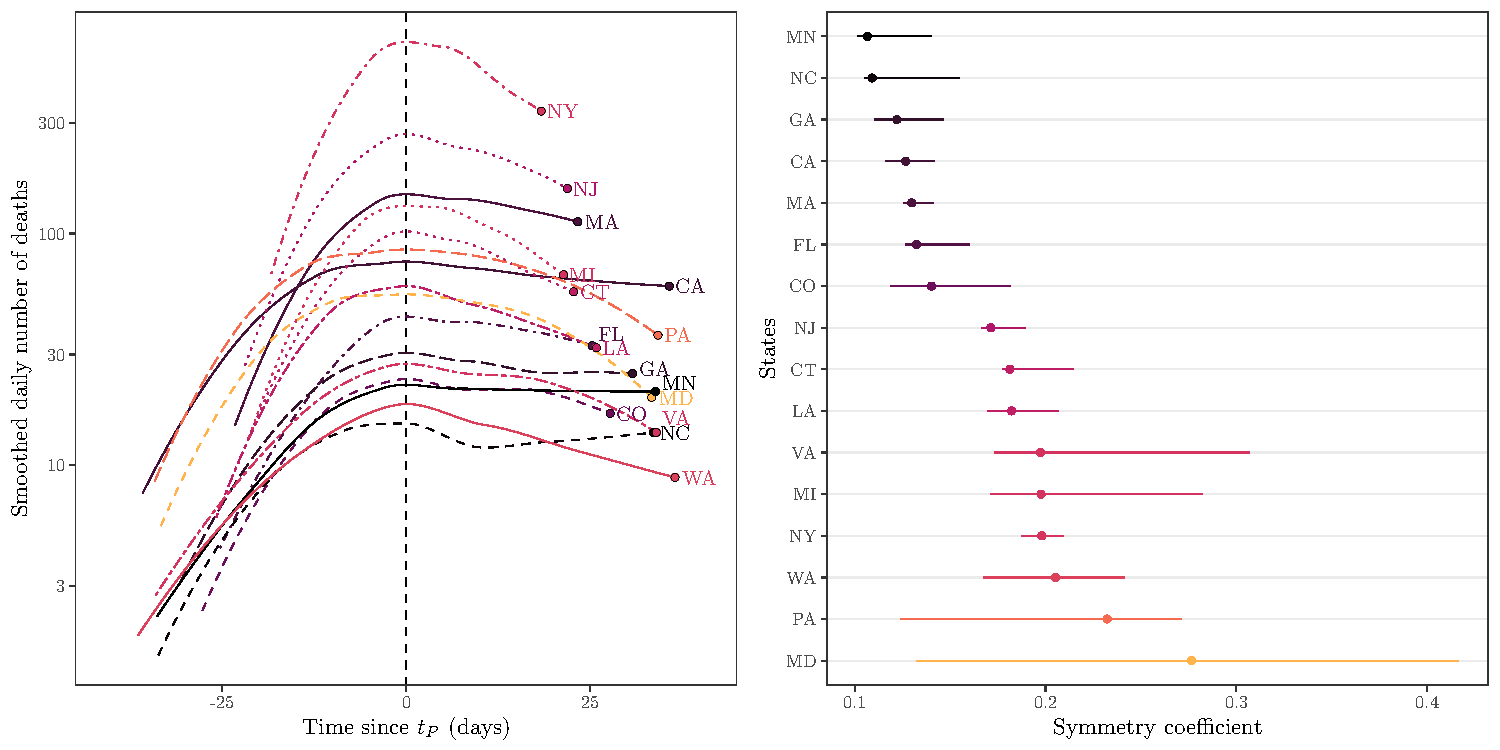
\includegraphics[width=0.9\textwidth]{deaths/national_deaths_metric_boot.pdf}\\
%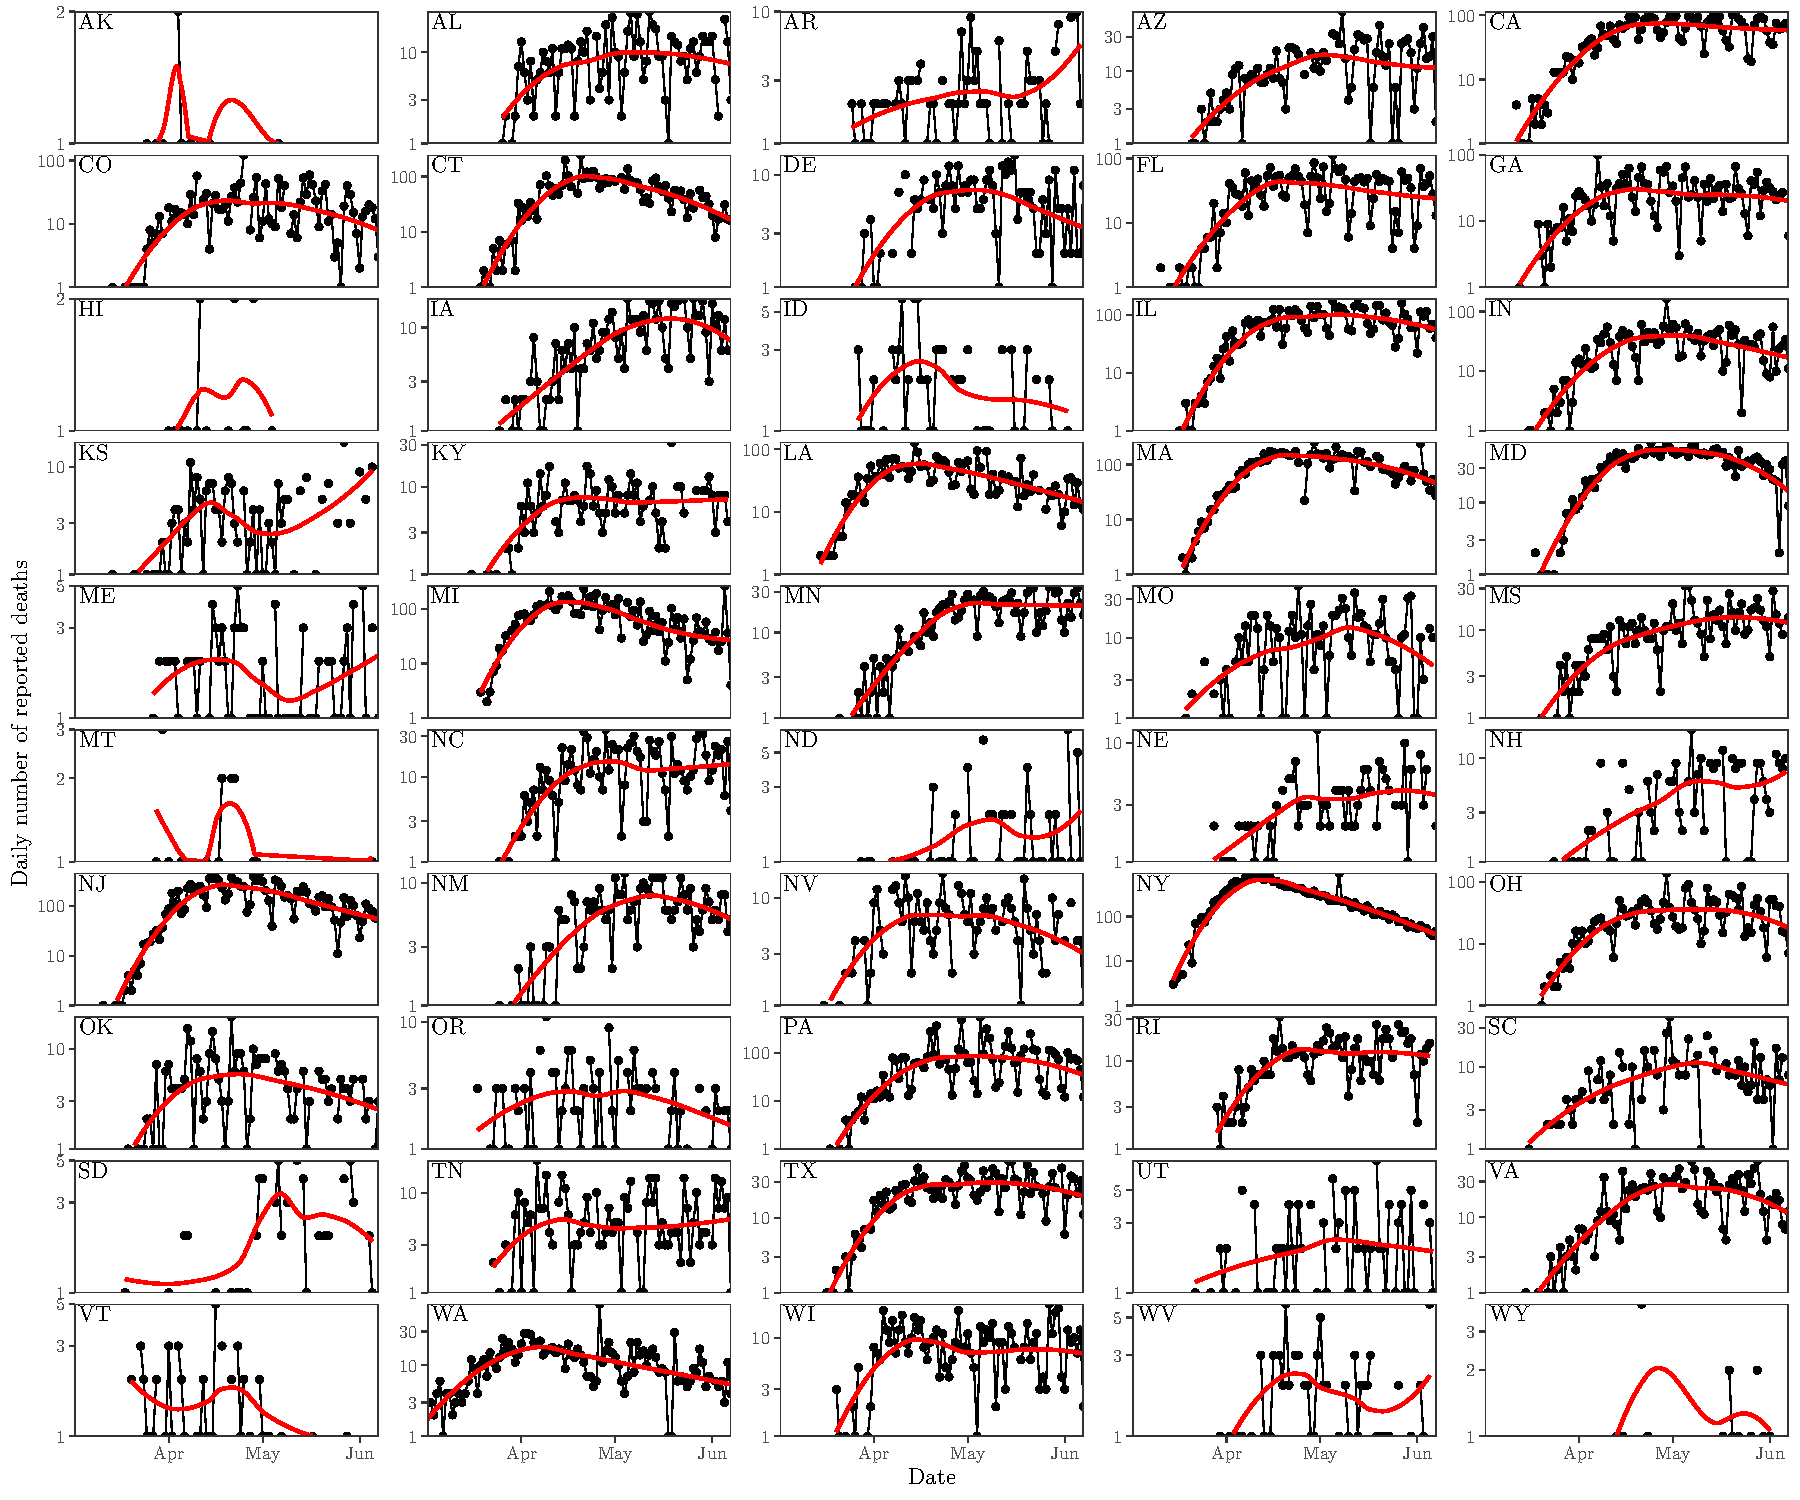
\includegraphics[width=0.9\textwidth]{deaths/deaths.pdf}
%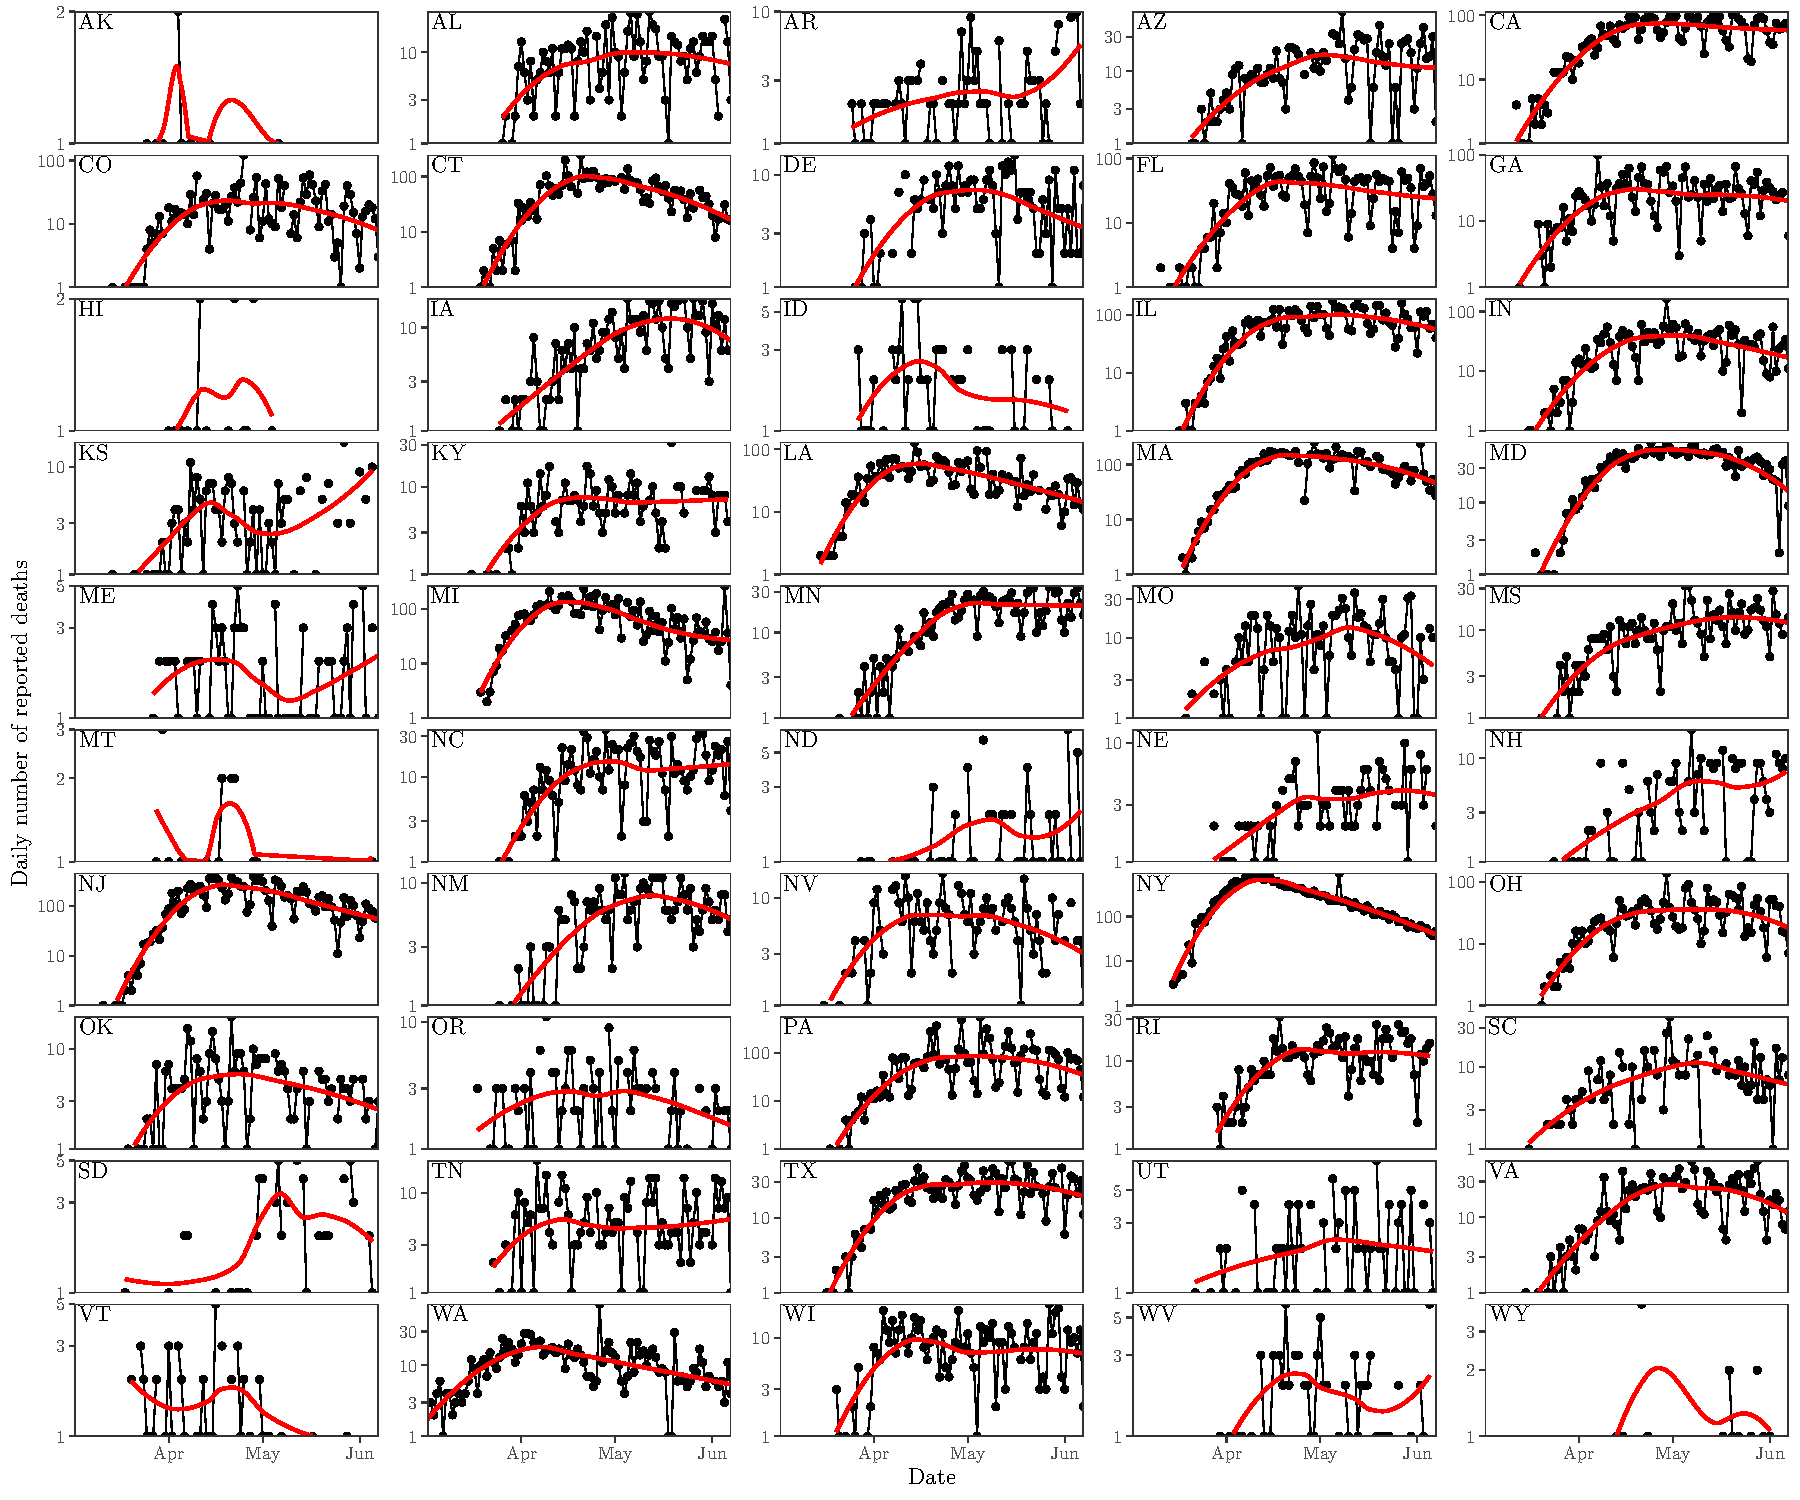
\includegraphics[width=0.8\textwidth]{deaths/deaths.pdf}
\caption{Plateaus and shoulder-like dynamics in 
COVID-19 fatalities.  
(A) Examples of daily number of reported deaths for COVID-19 (black points and lines) and the corresponding locally estimated scatterplot smoothing (LOESS) curves (red lines) in four states, including
two estimated to be the most plateau-like (Minnesota and North Carolina)
and two estimated to be the most peak-like (Indiana and Maryland). 
Daily number of deaths is smoothed in log space, only including days with one or more reported deaths.
We restrict our analysis to states in which the peak smoothed death is greater than 10 as of June 7, 2020 (resulting in 17 states in total).
(B) Smoothed daily number of reported deaths  centered around the first peak time $t_P$ across 17 states.
Smoothed death curves are plotted between $t_P - \Delta t$ and $t_P + \Delta t$, where $\Delta t$ is defined such that smoothed death at time $t_P - \Delta t$ corresponds to 10\% of the smoothed peak value.
(C) Measured symmetry coefficient and confidence intervals.
Symmetry coefficient is calculated by dividing the death value at time $t_P - \Delta t$ by the death value at time $t_P + \Delta t$. If the death curve is symmetric, the symmetry coefficient should equal 1.
Confidence intervals are calculated by bootstrapping across the date of deaths for each individual 1000 times and recalculating the symmetry coefficient (after smoothing each bootstrap time series).
LOESS smoothing is performed by using the \texttt{loess} function in \texttt{R}.
\label{fig.plateaus_cases}}
\end{center}
\end{figure*}

Conventional epidemic
models of COVID-19 represent populations in terms of their `status' vis
a vis the infectious agent, i.e., susceptible, exposed, infectious,
hospitalized, and recovered~\citep{ferguson2020report,kucharski2020early,kissler_medrxiv2020,park_medrxiv2020,kraemer_2020sci,li_science2020,wu_2020natmed}.
New transmission can lead to an exponential increases in cases 
when the basic reproduction number ${\cal{R}}_0>1$ (the
basic reproduction number denotes the average number of new
infections caused by a single, typical individual in an otherwise
susceptible population \citep{anderson1991infectious}).  Subsequent
spread, if left unchecked, would yield a single peak -- in theory. That 
peak corresponds to when `herd immunity' is reached, such
that the effective reproduction number, $\Reff=1$.
The effective reproduction number denotes the number of new
infectious cases caused by a single infectious individual
in a population with pre-existing circulation.
But, even when herd immunity is reached, there will still be new cases 
which then diminish over time, until the epidemic concludes.  
A single-peak paradigm is
robust insofar as the disease has spread
sufficiently in a population to reach and exceed `herd immunity'.
The converse
is also true  -- as long as 
a population remains predominantly immunologically
naive, then the risk of further infection has not passed. 

In contrast to the IHME model,
the Imperial College of London (ICL) model~\citep{ferguson2020report} 
used a conventional state-driven epidemic model
to show the benefits of  early intervention steps in reducing
transmission and preserving health system resources vs.~a `herd immunity' strategy.  
The ICL model assumed that
transmission is reduced because of externalities, like lockdowns,
school closings, and so on.  
As a result, early predictions of the ICL model suggested that lifting of large-scale
public health interventions could be followed by a second wave of cases.
This has turned out to be the case, in some jurisdictions.
Yet, for a disease
that is already the documented cause of more than 200,000 deaths
in the United States alone, we posit that individuals
are likely to continue to modify
their behavior even after lockdowns are lifted.  
Indeed, the peak death rates in the United States and globally
are not as high as potential maximums in the event that
COVID-19 had spread unhindered in the population~\citep{ferguson2020report}. 
Moreover, rather than a peak and symmetric decline, there is evidence 
%at both national
of asymmetric plateaus and shoulder-like
behavior for daily fatality rates in the spring-summer
trajectory of the pandemic in US-states
(Figure~\ref{fig.plateaus_cases}; full state-level data in Supplementary
Figure~\ref{fig.supp_plateaus}).  These early plateaus have
been followed, in many cases, with resurgence of cases and fatalities.  

In this manuscript we use a nonlinear model of epidemiological dynamics to
ask the question: what is the anticipated
shape of an epidemic if individuals modify their behavior in direct
response to the impact of a disease at the population level? In doing so,
we build upon earlier work on awareness based models (e.g.~\citep{funk2009spread,funk2010modelling,eksin2017disease, eksin2019systematic}) with an
initial assumption: individuals reduce interactions when 
death rates are high and increase interactions when death rates are low.  
As we show, short-term awareness can lead to dramatic reductions
in death rates compared to models without accounting for behavior,
leading to plateaus, shoulders,
and lag-driven oscillations in death rates. We also show that dynamics
can be driven from persistent dynamics to elimination when
awareness shifts from short- to long-term. Notably, we find
that despite model predictions, the empirical data reveals
that mobility increased even as fatalities were increasing. 
This reveals the potential role for fatigue and long-term
changes in behavior beyond those linked to mobility (e.g., mask-wearing)
in shaping Covid-19 dynamics.

\section{Results and Discussion}

\begin{table}[!h]
\begin{tabular}{l|p{3cm}|l}
\hline
Notation & Description & Values/Ranges\\
\hline
$\beta$ & Transmission rate & 1/2 days$^{-1}$ \\
$1/\mu$ & Mean latent period & 2 days \\
$1/\gamma$ & Mean infectious period & 6 days \\
$1/\gamma_H$ & Mean time in a hospital stay before a fatality & 7--28 days\\
$f_D$ & infection fatality probability & 0.01 \\
$N$ & Population size & $10^7$ \\
$N\delta_c$ & Half-saturation constant for short-term awareness & 5--500 deaths/day \\
$ND_c$ & Half-saturation constant for long-term awareness & 2,500--10,000 deaths \\
$k$ & sharpness of change in the force of infection & 1--4 \\
$\epsilon$ & Time scale of behavior change & 1/7 days$^{-1}$\\
\hline
\end{tabular}
\caption{
Parameter descriptions and values/ranges used for simulations. Transmission rate is chosen to match $\mathcal{R}_0 = 3$.
}
\end{table}

\subsection{SEIR Model with Short-Term Awareness of Risk}
Consider an SEIR like model
\begin{eqnarray}
\dot{S} &=& -\frac{\beta SI}{\left[1+\left(\delta/\delta_c\right)^{k}\right]}\\
\dot{E} &=& \frac{\beta SI}{\left[1+\left(\delta/\delta_c\right)^{k}\right]}-\mu E\\
\dot{I} &=& \mu E-\gamma I \\
\dot{R} &=& (1-f_D)\gamma I\\
\dot{D} &=& f_D\gamma I
\end{eqnarray}
%\begin{eqnarray}
%\dot{S} &=& -\beta SI a(\vec{x}) \\
%\dot{E} &=& \beta SI} a(\vec{x})}-\mu E\\
%\dot{I} &=& \mu E-\gamma I \\
%\dot{R} &=& (1-f_D)\gamma I
%\dot{D} &=& f_D)\gamma I
%\end{eqnarray}
%where $a(\vec{x})$ denotes awareness-based distancing given the
%epidemiological phase space
where $S$, $E$, $I$, $R$, and $D$ denote the proportions of
susceptible, exposed, infectious, recovered, and deaths, respectively,
given transmission rate $\beta$ /day, transition
to infectious rate $\mu$ /day, recovery rate $\gamma$ /day,
where $f_D$ is the infection fatality probability.
The awareness-based distancing is controlled by 
the death rate $\delta\equiv \dot{D}$,
the half-saturation constant ($\delta_c>0$), and
the sharpness of change in the force of infection ($k\geq 1$)
(see Figure~\ref{fig.schematic} for a schematic).
Since $\delta$ is proportional to $I$, this model is closely related to a recently proposed awareness-based distancing model~\citep{eksin2019systematic}
and to an independently derived feedback SIR model~\citep{franco2020feedback}.
Note that the present
model converges to the conventional SEIR model as $\delta_c\rightarrow \infty$.
\begin{figure}[t!]
\begin{center}
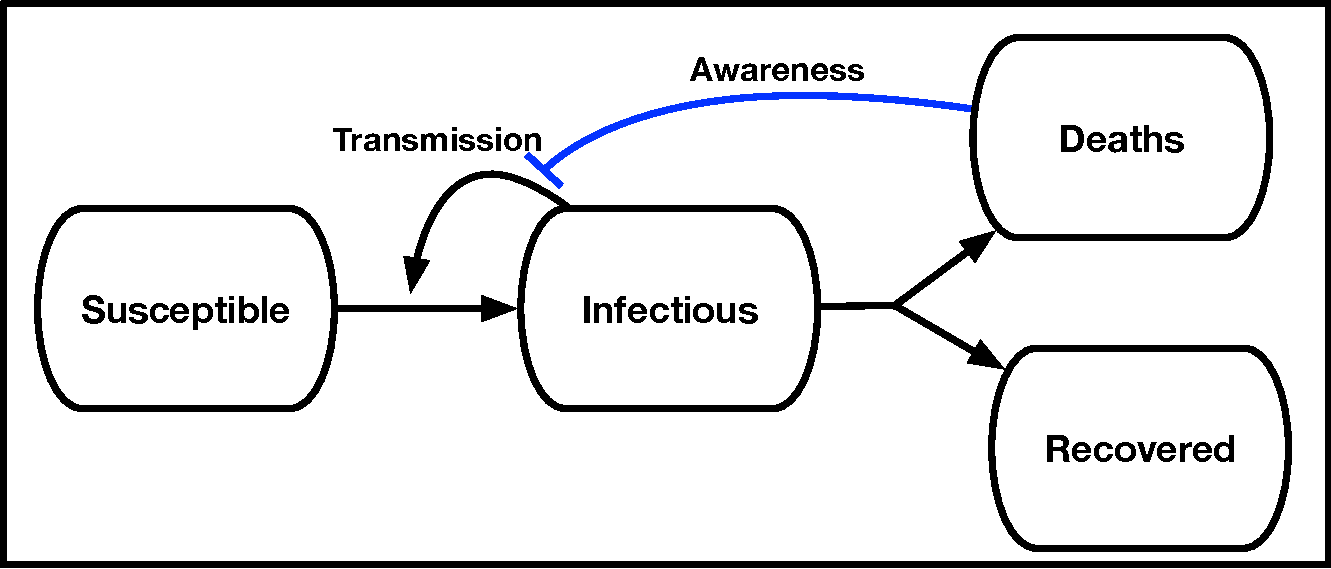
\includegraphics[width=0.475\textwidth]{schematics/plateau_schematic.pdf}
\caption{Schematic of an SEIR model with awareness-driven social distancing.
Transmission is reduced based on short- and/or long-term awareness
of population-level disease severity (i.e., fatalities).
\label{fig.schematic}}
\end{center}

\end{figure}
\begin{figure}[t!]
\begin{center}
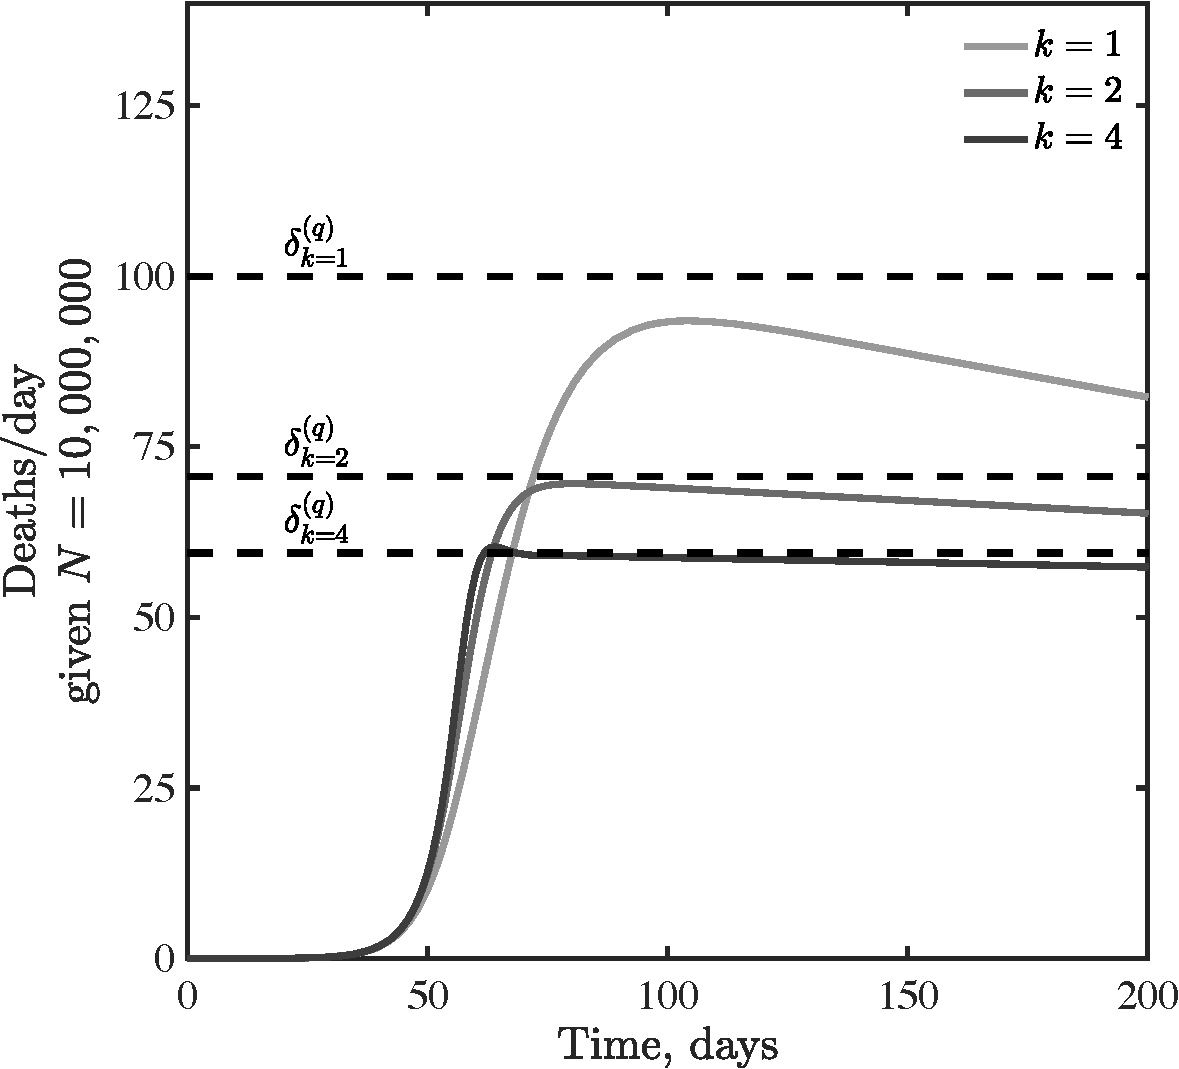
\includegraphics[width=0.4\textwidth]{scripts/figseir_baseplat_k2_D_noname.pdf}\\
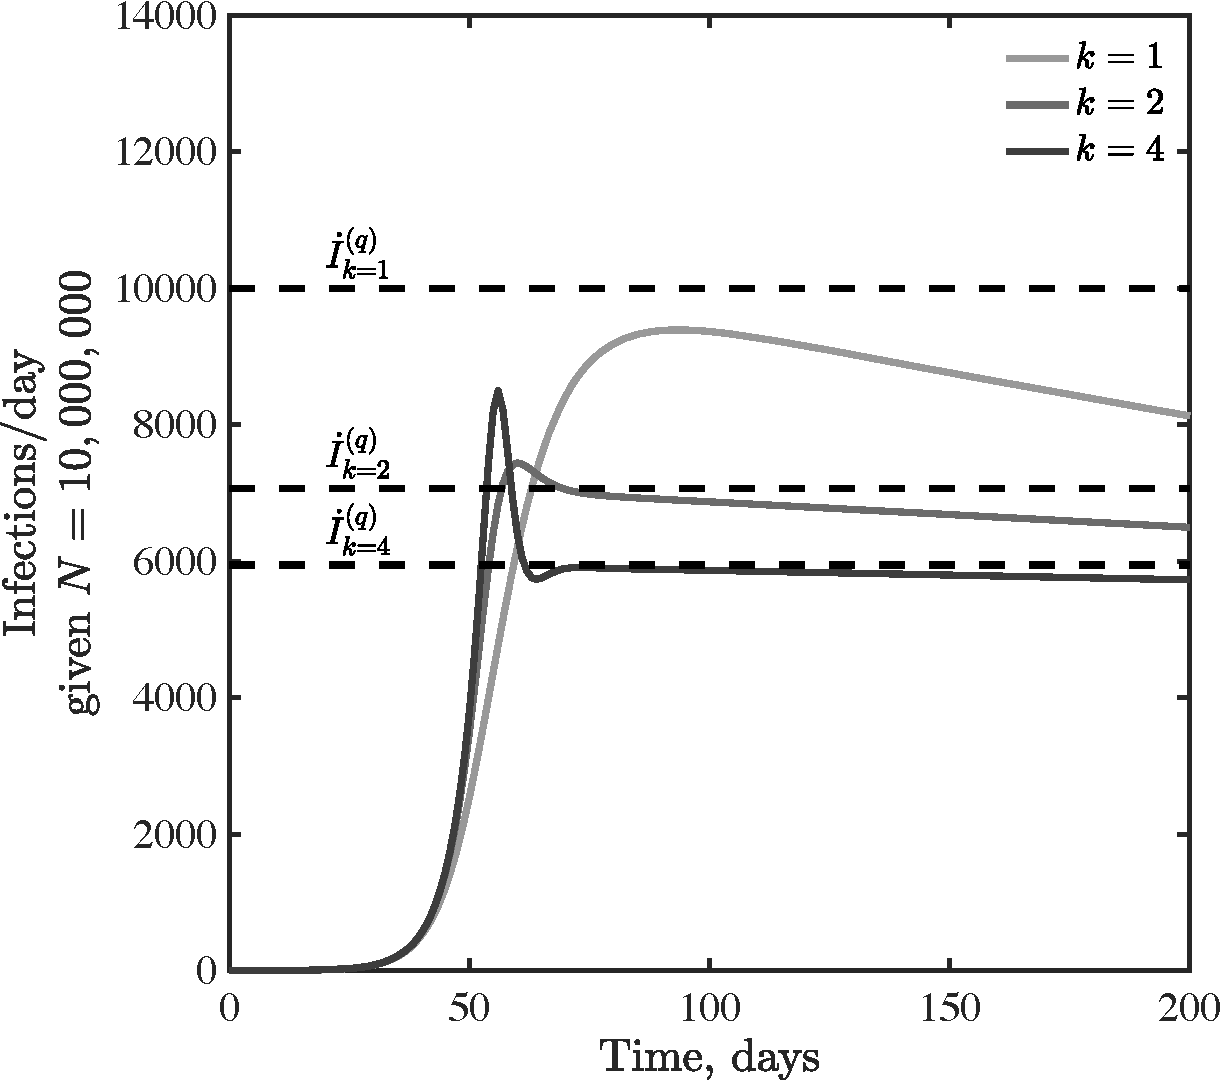
\includegraphics[width=0.4\textwidth]{scripts/figseir_baseplat_k2_I_noname.pdf}
\caption{Infections and deaths per day in a death-awareness based
social distancing model.  Simulations have the
epidemiological parameters 
$\beta=0.5$ /day, $\mu=1/2$ /day, $\gamma=1/6$/day,
and $f_D=0.01$, with variation in $k=1$, 2 and 4. We assume
$N\delta_c = 50$ /day in all cases.
\label{fig.ID_day}}
\end{center}
\end{figure}

\begin{figure}[t!]
\begin{center}
%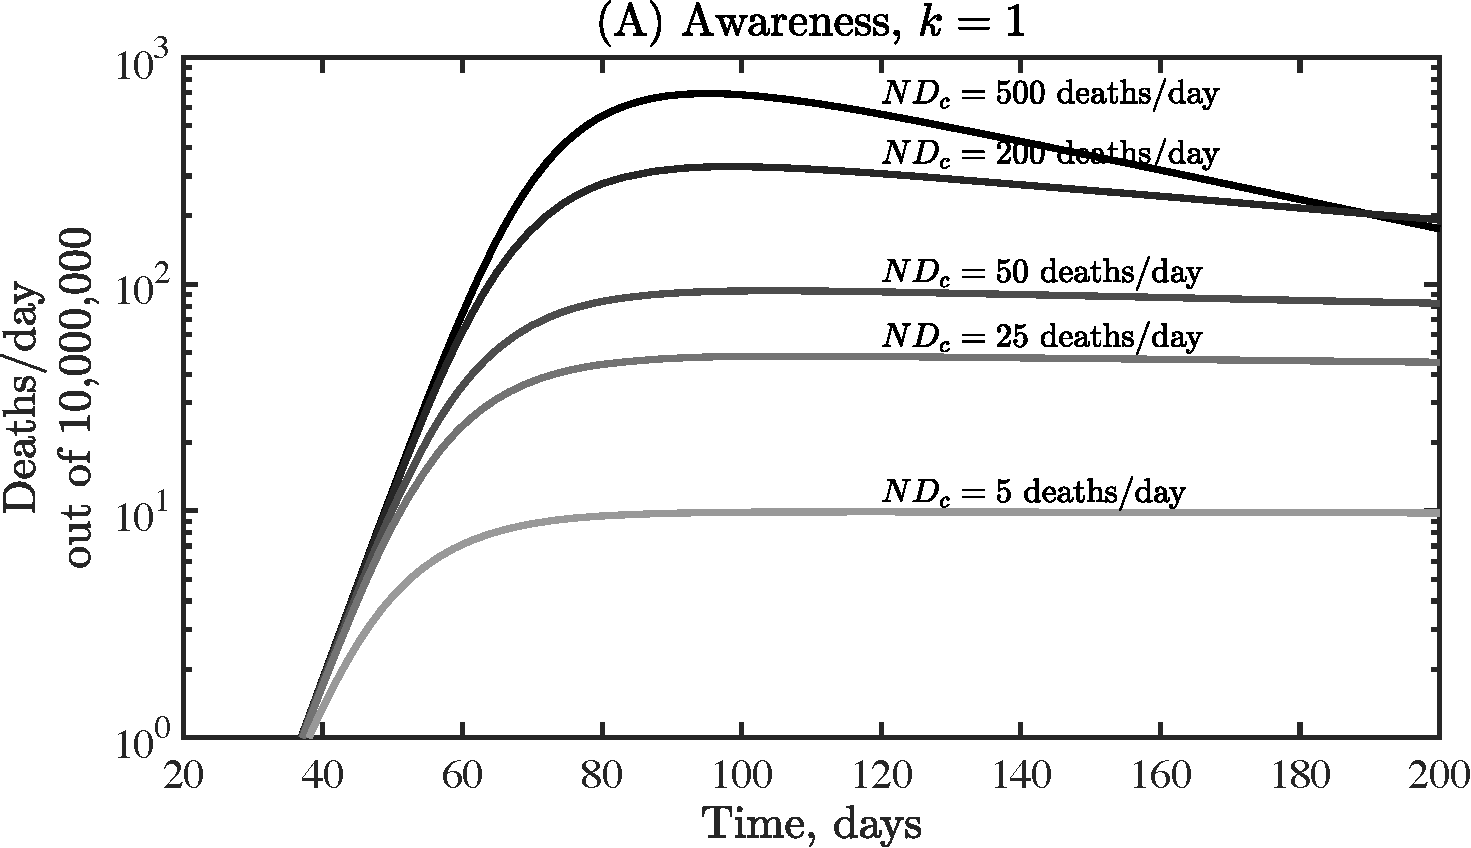
\includegraphics[width=0.45\textwidth]{figseir_Speak_k1_noname.pdf}
%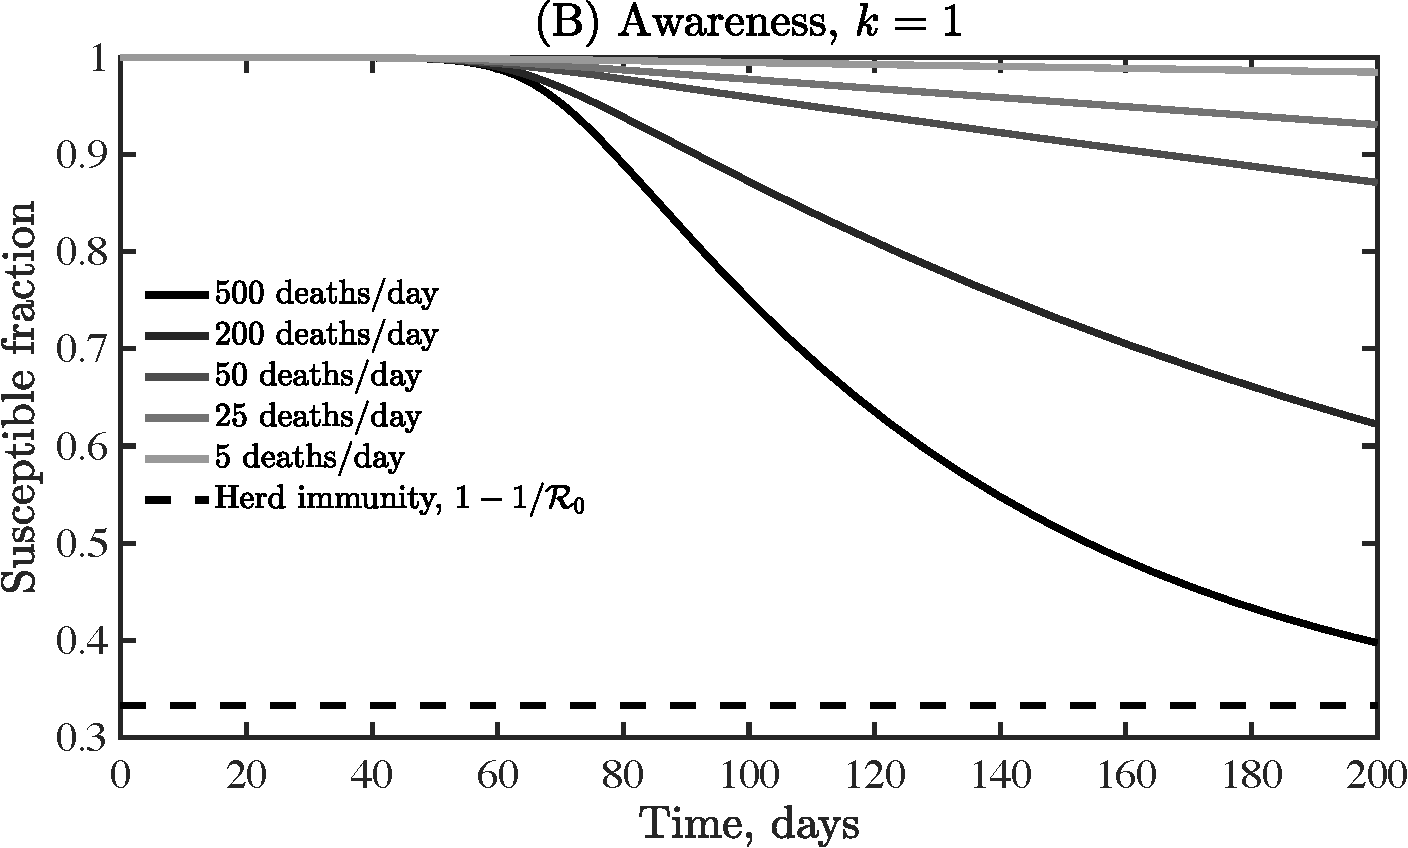
\includegraphics[width=0.435\textwidth]{figseir_Susc_k1_noname.pdf}\\
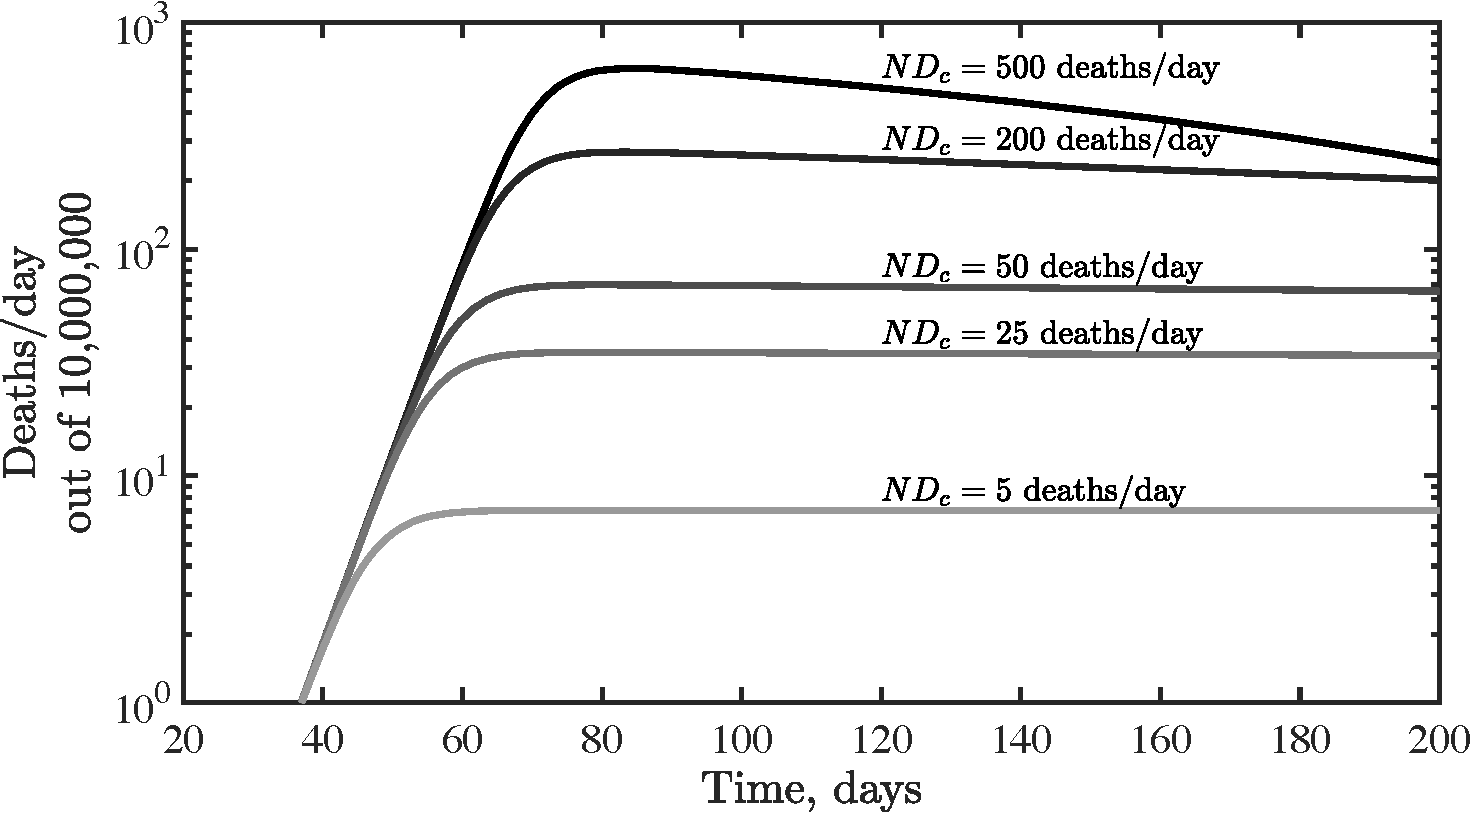
\includegraphics[width=0.4\textwidth]{scripts/figseir_Speak_k2_noname.pdf}\\
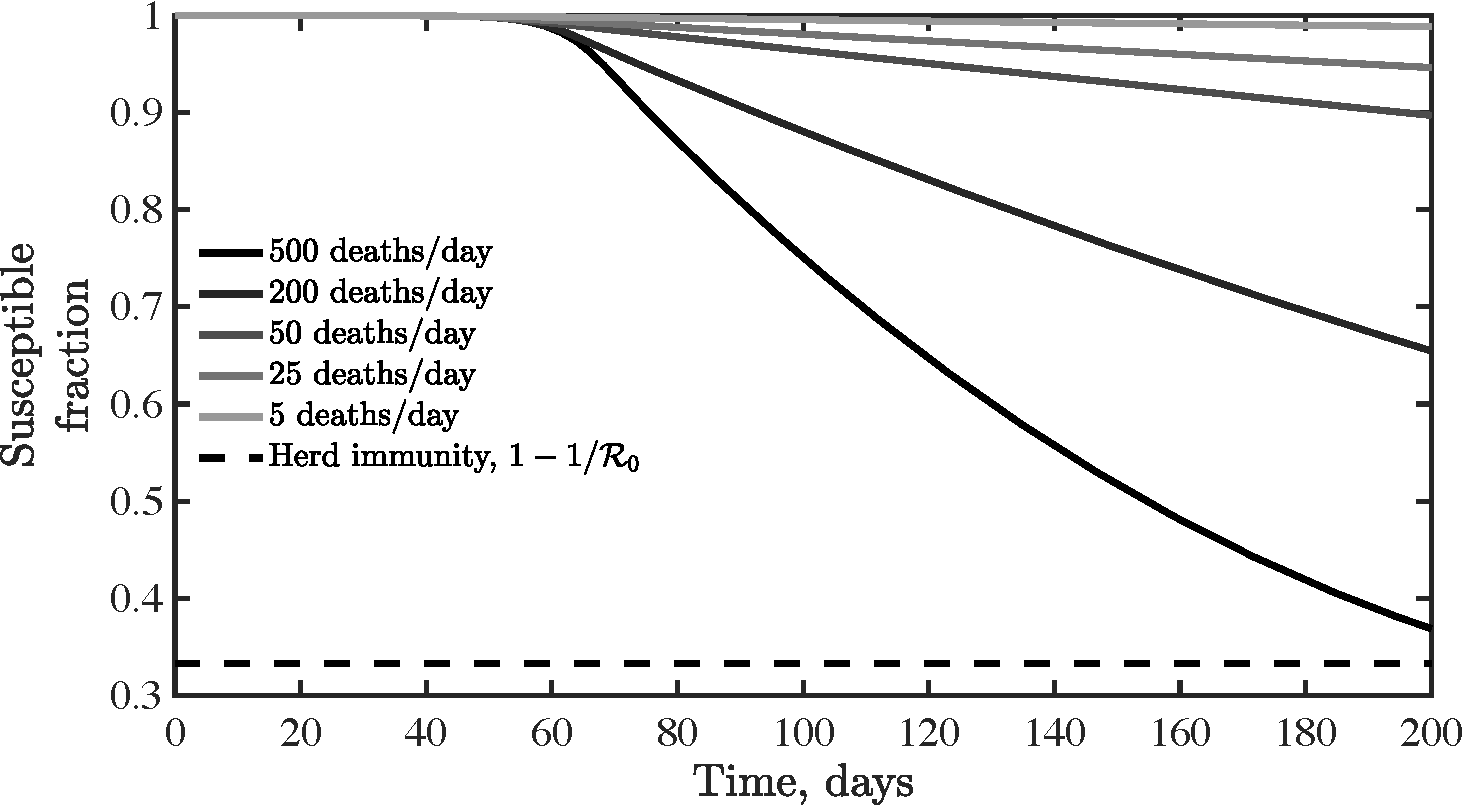
\includegraphics[width=0.4\textwidth]{scripts/figseir_Susc_k2_noname.pdf}
%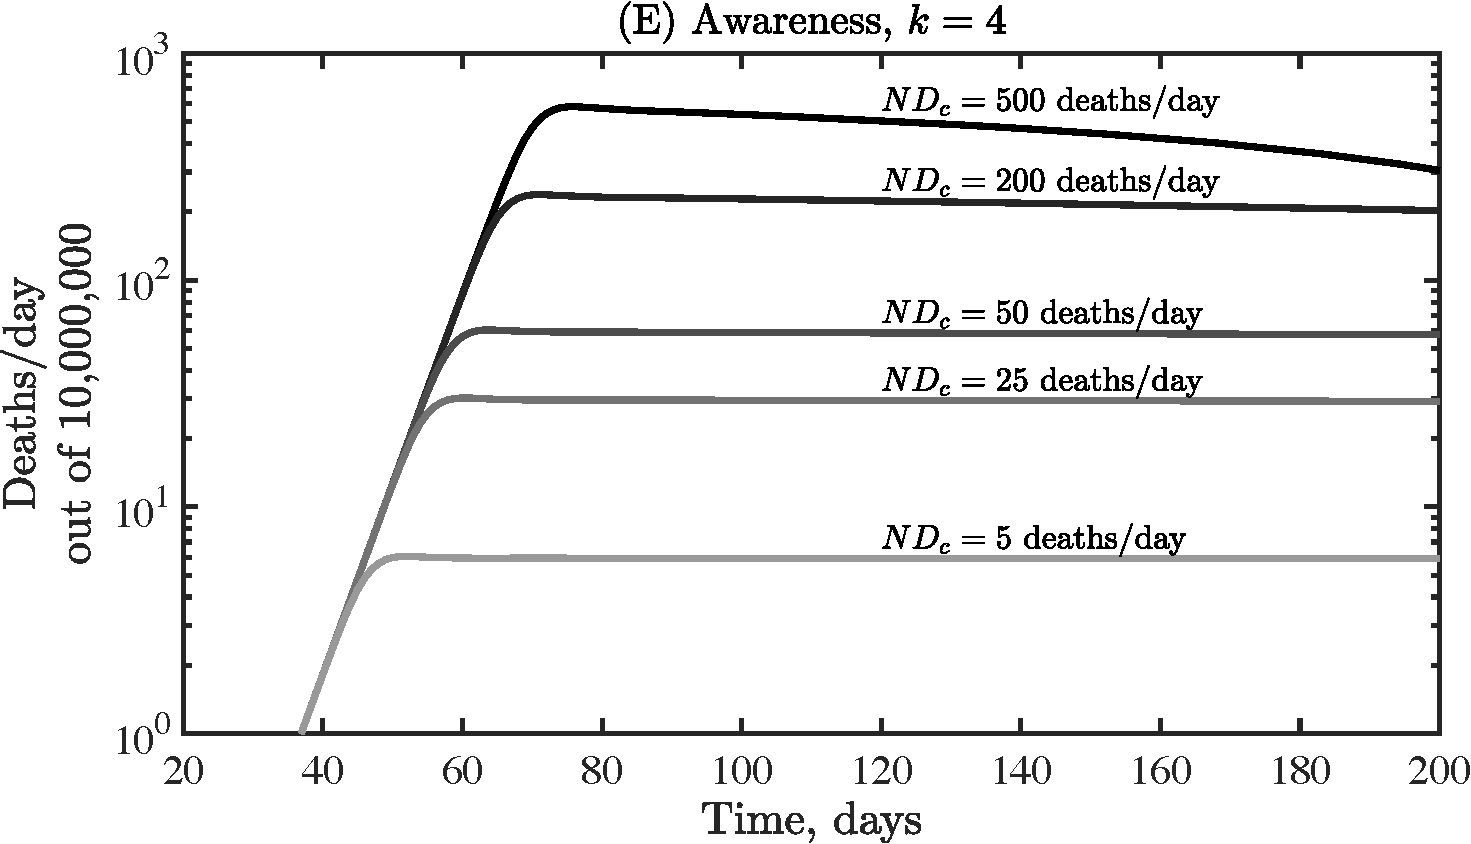
\includegraphics[width=0.45\textwidth]{figseir_Speak_k4_noname.pdf}
%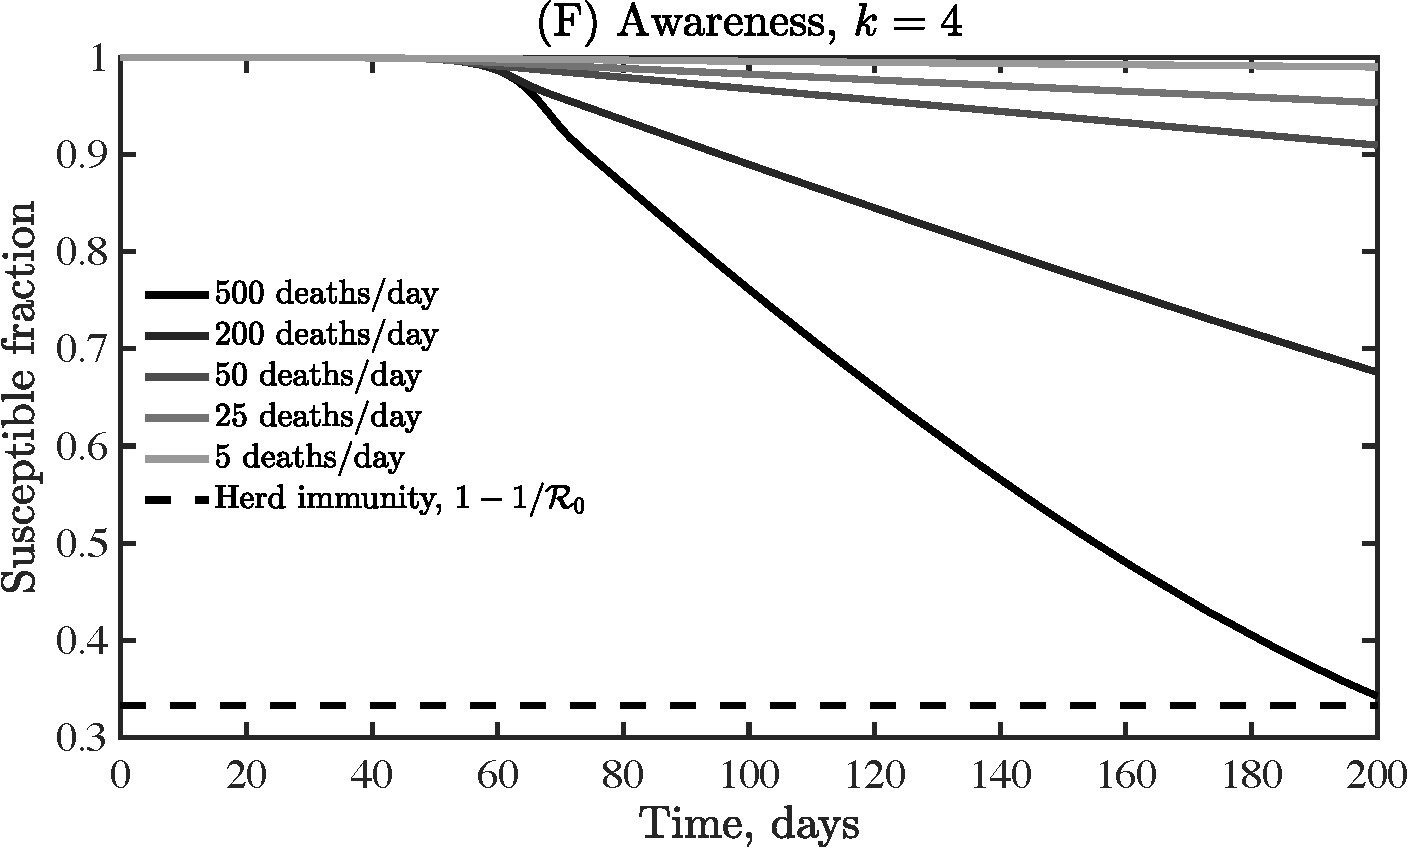
\includegraphics[width=0.435\textwidth]{figseir_Susc_k4_noname.pdf}\\
\caption{Dynamics given variation in the critical fatality awareness
level, $\delta_c$ for awareness $k=2$. Panels show
deaths/day (top) and the susceptible fraction as a function of time (bottom),
the latter compared to a herd immunity
level when only a fraction $1/{\cal{R}}_0$ remain susceptible.
These simulations share the
epidemiological parameters 
$\beta=0.5$ /day, $\mu=1/2$ /day, $\gamma=1/6$ /day,
and $f_D=0.01$.
\label{fig.generic}}
\end{center}
\end{figure}

Uncontrolled epidemics in SEIR models have a single case peak, corresponding 
to the point where $\gamma I = \beta S I $ such that 
the population obtains herd immunity when only a proportion
$S=1/{\cal{R}}_0$ have yet to be infected.
However, in the model above individuals decrease transmission in response
to awareness of the impacts of the disease, $\delta(t)$.
In this case, the the system can peak when levels of infected cases are
far from herd immunity, specifically when
\begin{equation}
\gamma I = \frac{\beta SI}{\left[1+\left(\delta/\delta_c\right)^{k}\right]}.
\end{equation}
When $\delta_c$ is small compared to the per-capita death rate of infectious individuals $(\gamma f_D)$ we anticipate that individual behavior will respond quickly to the disease outbreak.
Hence, we hypothesize that the
emergence of an
awareness-based peak can occur early, i.e., $S(t)\approx 1$, consistent
with a quasi-stationary equilibrium when the death rate is
\begin{equation}
\delta^{(q)} \approx \delta_c\left({\cal{R}}_0-1\right)^{1/k}
\end{equation}
and the infection rate is
\begin{equation}
\dot{I}^{(q)} \approx \frac{\delta_c}{f_D}\left({\cal{R}}_0-1\right)^{1/k}.
\end{equation}
These quasi-equilibrium is maintained not because of herd immunity, but because of changes in behavior. 

We evaluate this hypothesis in
Figure~\ref{fig.ID_day} for $k=1$, $k=2$, and $k=4$
given disease dynamics with $\beta=0.5$/day, $\mu=1/2$/day, $\gamma=1/6$/day,
$f_D=0.01$, $N=10^7$, and $N\delta_c=50$/day.  
As is evident, the rise and decline from peaks are not symmetric. Instead,
incorporating
awareness leads to dynamics where incidence decreases very slowly after a peak.
The peaks occur at levels of infection far from that associated
with herd immunity.  
Post-peak, shoulders and plateaus emerge because of the balance
between relaxation of awareness-based
distancing (which leads to increases in cases and deaths) and an 
increase in awareness in response to increases in cases and deaths.  
As the steepness of response $k$ increases, 
individuals become less sensitive to fatality rates
where $\delta < \delta_c$ and more sensitive to fatality rates where $\delta > \delta_c$.  
This leads to sharper dynamics. In addition, 
infections can over-shoot the expected plateau given that awareness
is driven by fatalities which are offset with respect to new infections.

\subsection{Short-term awareness, long-term plateaus, and oscillations}
Initial analysis of an SEIR model with short-term 
awareness of population-level severity suggests a generic outcome: 
fatalities will first increase exponentially before before slowing to plateau at a level near $\delta_c$.
Figure~\ref{fig.generic} shows dynamics for values of $\delta_c$ ranging 
from to 5 to 500 deaths/day in a population of $10^7$
(here $k=2$; results for $k=1$ or $k=4$ are similar, see Figure~\ref{fig.generic_k1-4}).
When $\delta_c$ is small (compared to $(\gamma f_D)$, fatalities can be sustained at near-constant levels for a long time.
When $\delta_c$ is higher then the decline of cases and fatalities due to susceptible depletion is relatively fast.
However, over a wide range of assumptions about critical daily fatality rates $\delta_c$, the population remains largely susceptible even as sustained fatalities continue for a period far greater than
the time it took to reach the plateau.
%We also observe that as $k$ increases, then fatalities may overshoot
%the plateau. Overshoots arise because individuals initiate protective measures
%closer to the critical fatality rate.
%These overshoots may lead to oscillatory dynamics
%when there are larger lags between new cases and fatalities.

%\subsection{Emergent oscillations given lags between cases and fatalities}
To explore the impacts of lags on dynamics,
we incorporated an additional class $H$,
assuming that fatalities follow potentially prolonged
hospital stays.  We do not include 
detailed information on symptomatic transmission, asymptomatic
transmission, hospitalization outcome,
age structure, and age-dependent risk (as in~\citep{ferguson2020report}). 
Instead, we consider the extended SEIR model:
\begin{eqnarray}
\dot{S} &=& -\frac{\beta SI}{\left[1+\left(\delta/\delta_c\right)^{k}\right]}\\
\dot{E} &=& \frac{\beta SI}{\left[1+\left(\delta/\delta_c\right)^{k}\right]}-\mu E\\
\dot{I} &=& \mu E-\gamma I \\
\dot{R} &=& (1-f_D)\gamma I\\
\dot{H} &=& f_D\gamma I - \gamma_H H\\
\dot{D} &=& \gamma_H H
\end{eqnarray}
where $T_H=1/\gamma_H$ defines the average time in a hospital
stay before a fatality. Note, we recognize that many individuals
recover from COVID-19 after hospitalization; this model's hospital
compartment functions as a prefilter.  

The earlier analysis of
the quasi-stationary equilibrium in fatalities holds in the
case of a SEIR model with additional classes before
fatalities. Hence,
we anticipate that dynamics should converge to $\delta=\delta^{(q)}$
at early times. However, increased delays between cases and
fatalities could lead to oscillations.  Indeed, this
is what we find via examination of models in which
$T_H$ ranges from 7 to 28 days, with increasing magnitude of
oscillations as $T_H$ increases (see Figure~\ref{fig.oscillate} 
for $k=2$ with qualitatively similar results for $k=1$ and
$k=4$ shown in Figure~\ref{fig.oscillate_k1-4}).

\begin{figure}[t!]
\begin{center}
%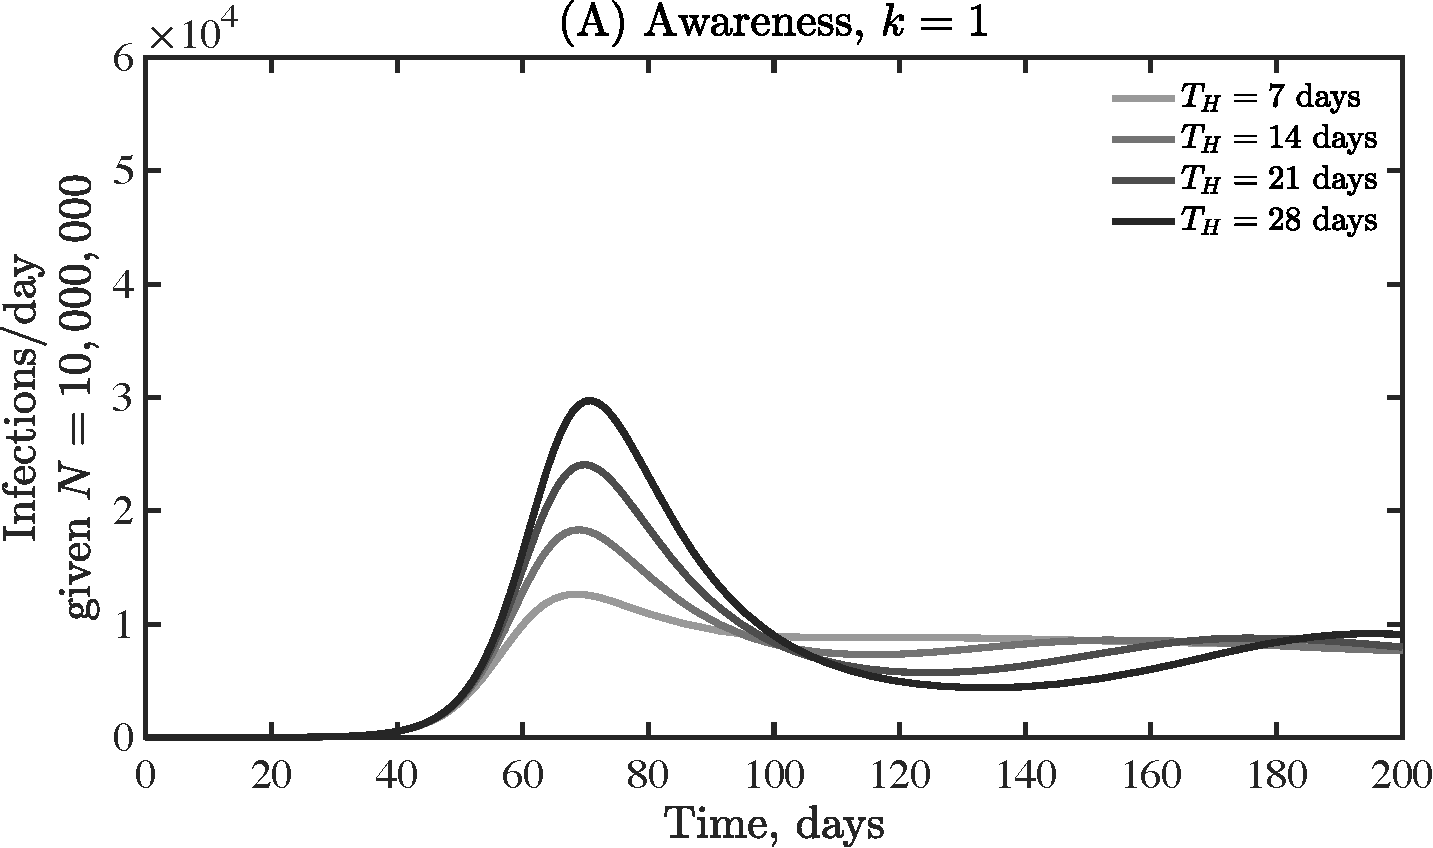
\includegraphics[width=0.45\textwidth]{figseir_Hdel_k1_noname.pdf}
%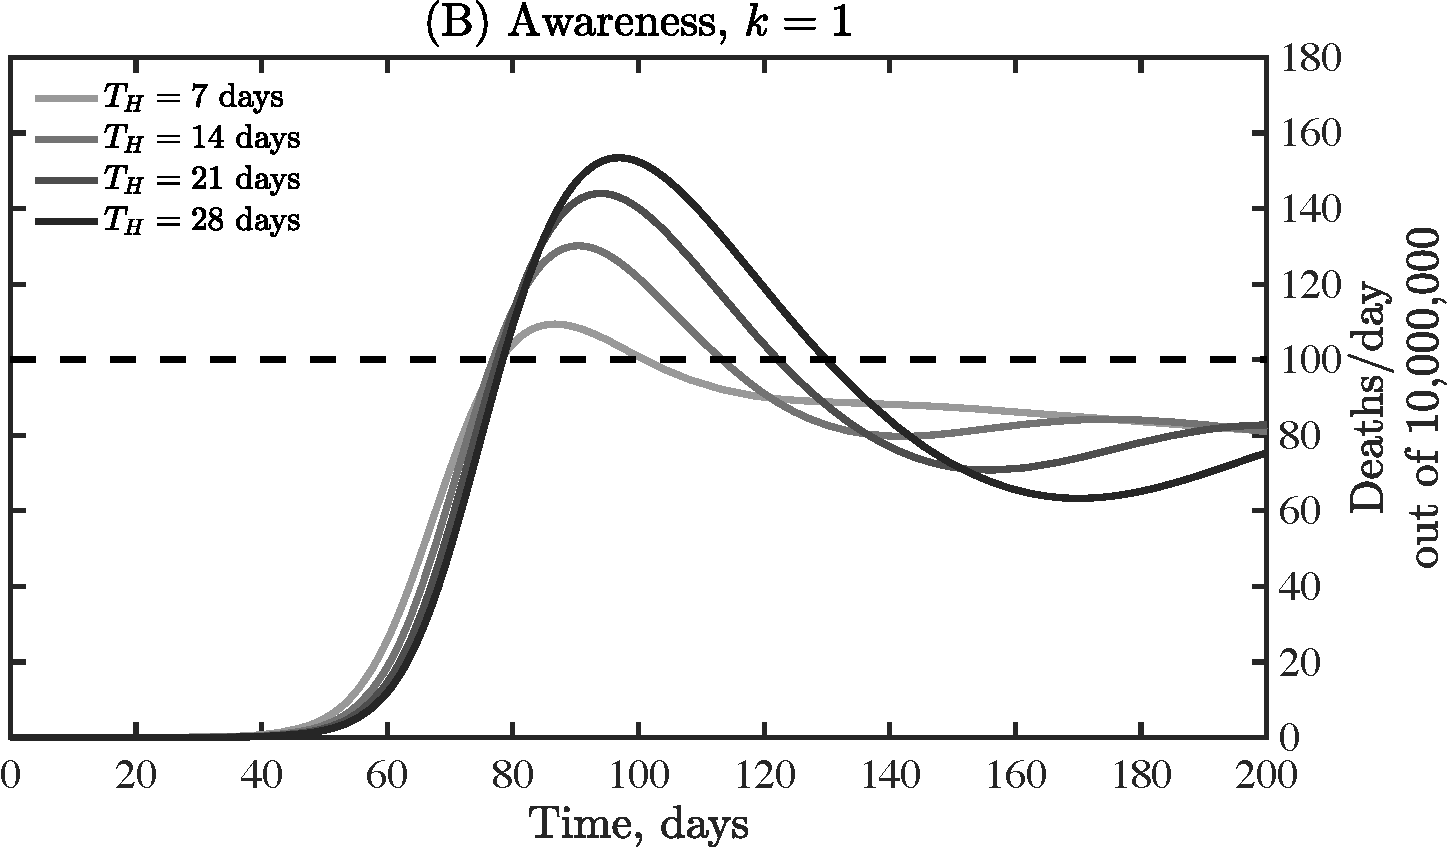
\includegraphics[width=0.45\textwidth]{figseir_Hdel_k1D_noname.pdf}\\
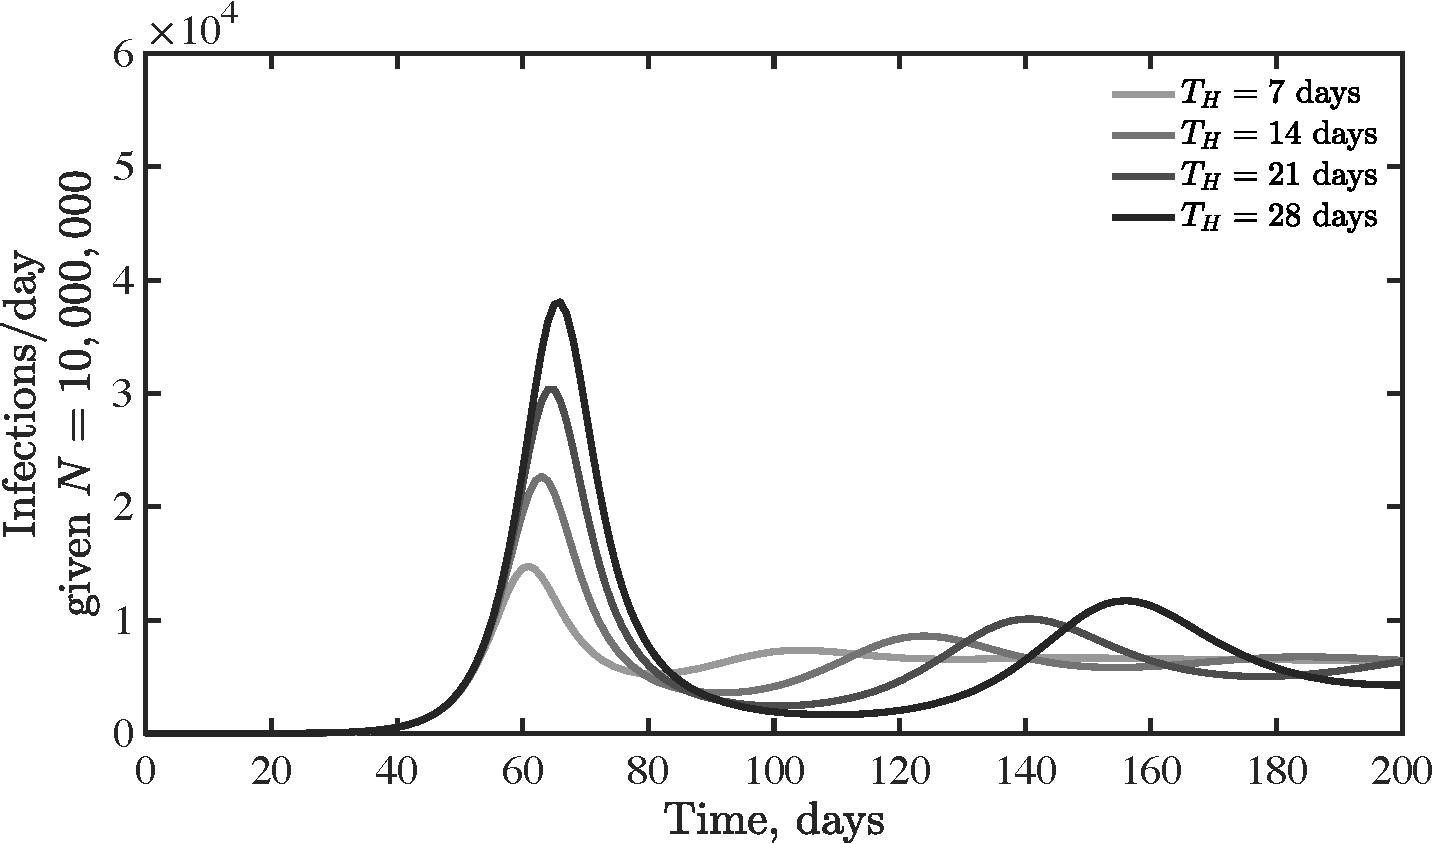
\includegraphics[width=0.47\textwidth]{scripts/figseir_Hdel_k2_noname.pdf}\\
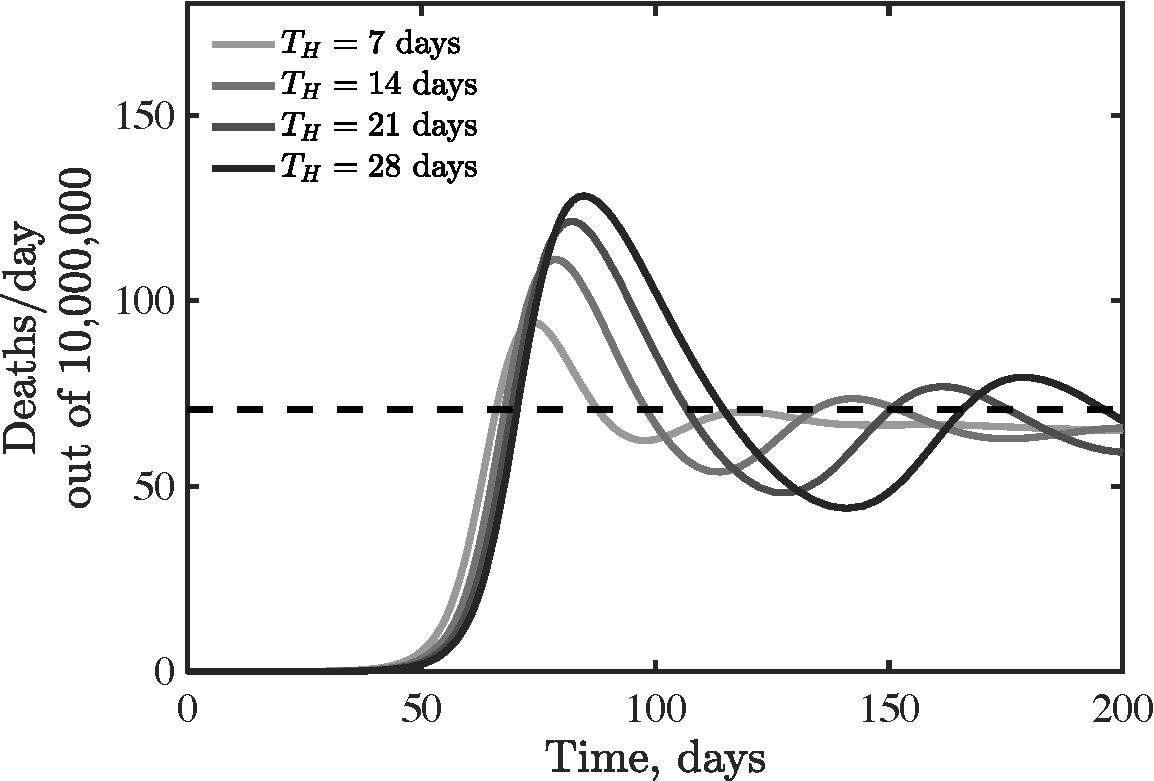
\includegraphics[width=0.47\textwidth]{scripts/figseir_Hdel_k2D_noname.pdf}
%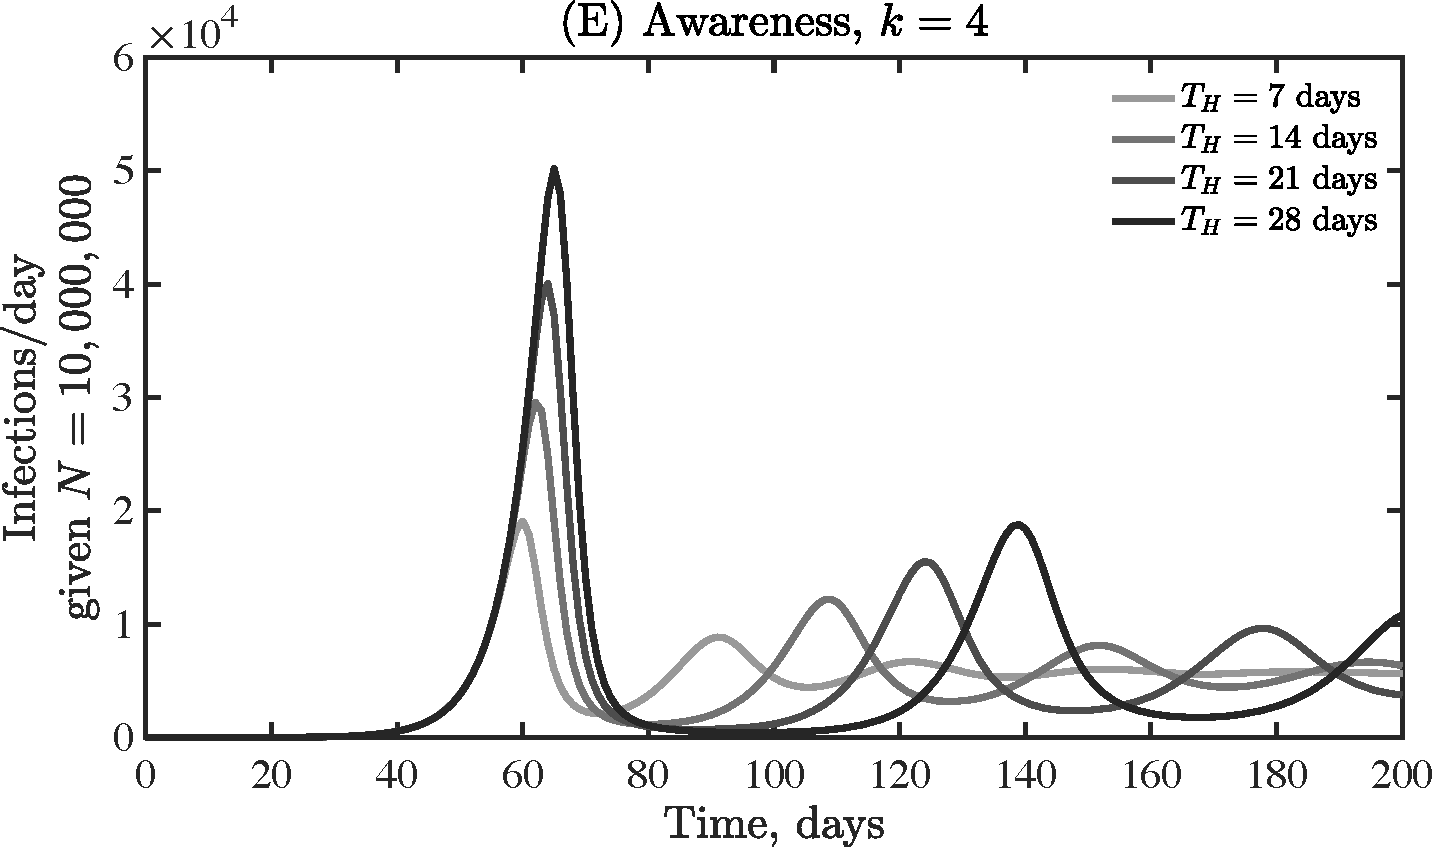
\includegraphics[width=0.45\textwidth]{figseir_Hdel_k4_noname.pdf}
%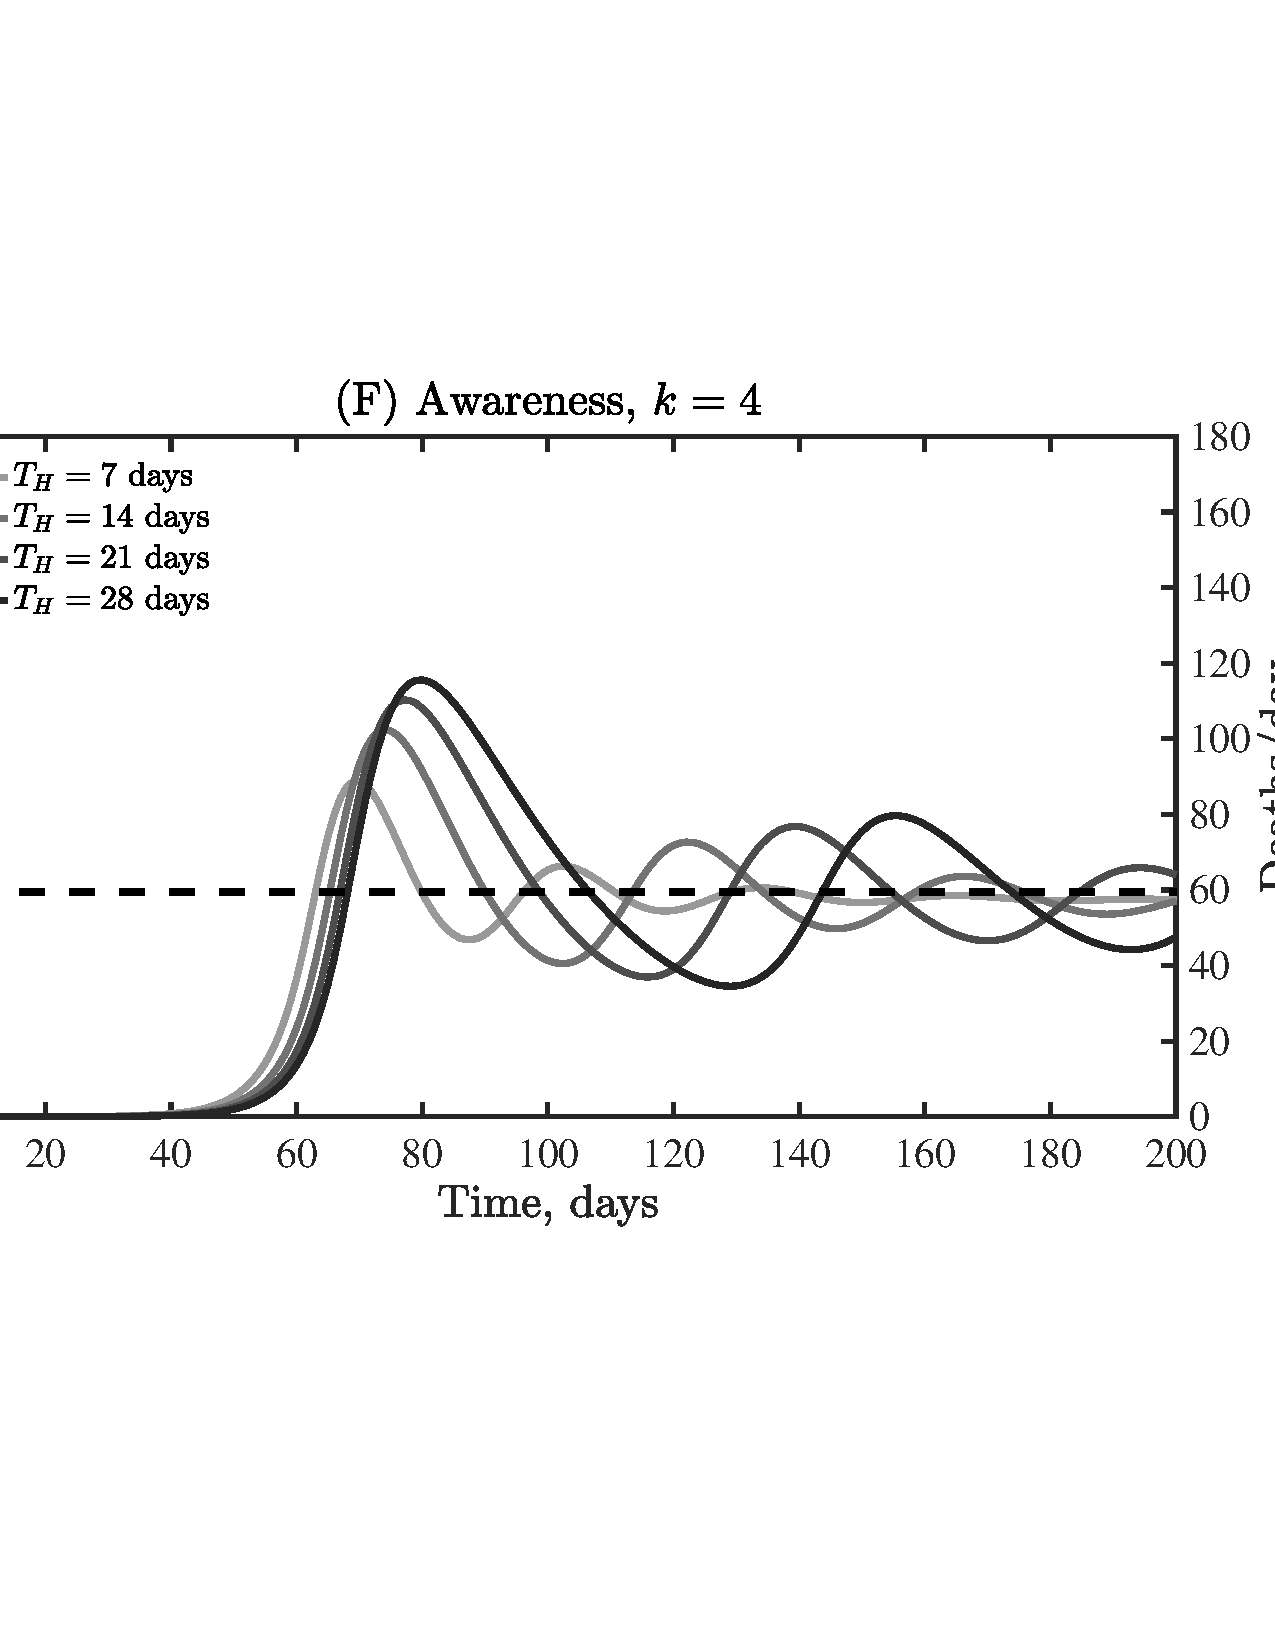
\includegraphics[width=0.45\textwidth]{figseir_Hdel_k4D_noname.pdf}\\
\caption{Emergence of oscillatory dynamics in a death-driven awareness
model of social distancing given lags between infection and fatality.
Awareness is $k=2$ and all other parameters as in Figure~\ref{fig.ID_day}.
The dashed
lines for fatalities expected quasi-stationary value $\delta^{(q)}$.
\label{fig.oscillate}}
\end{center}
\end{figure}

\begin{figure}[t!]
\begin{center}
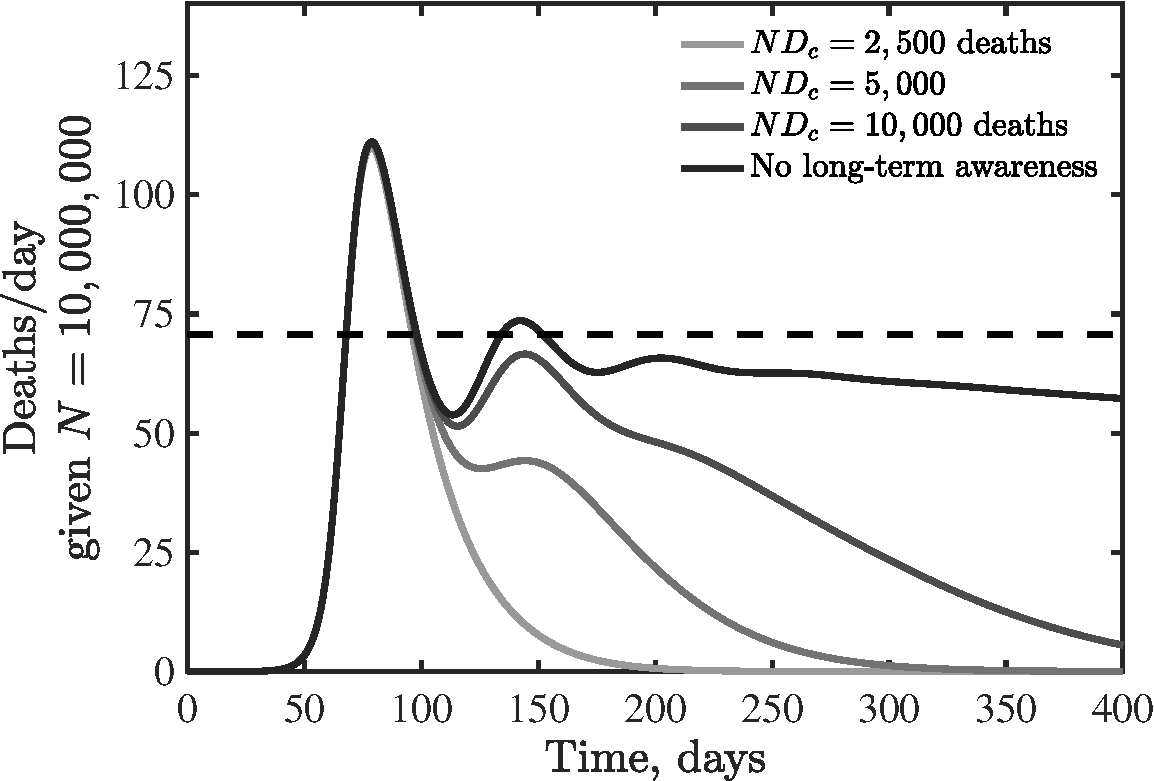
\includegraphics[width=0.47\textwidth]{scripts/figseir_Hlong_k2D_noname.pdf}\\
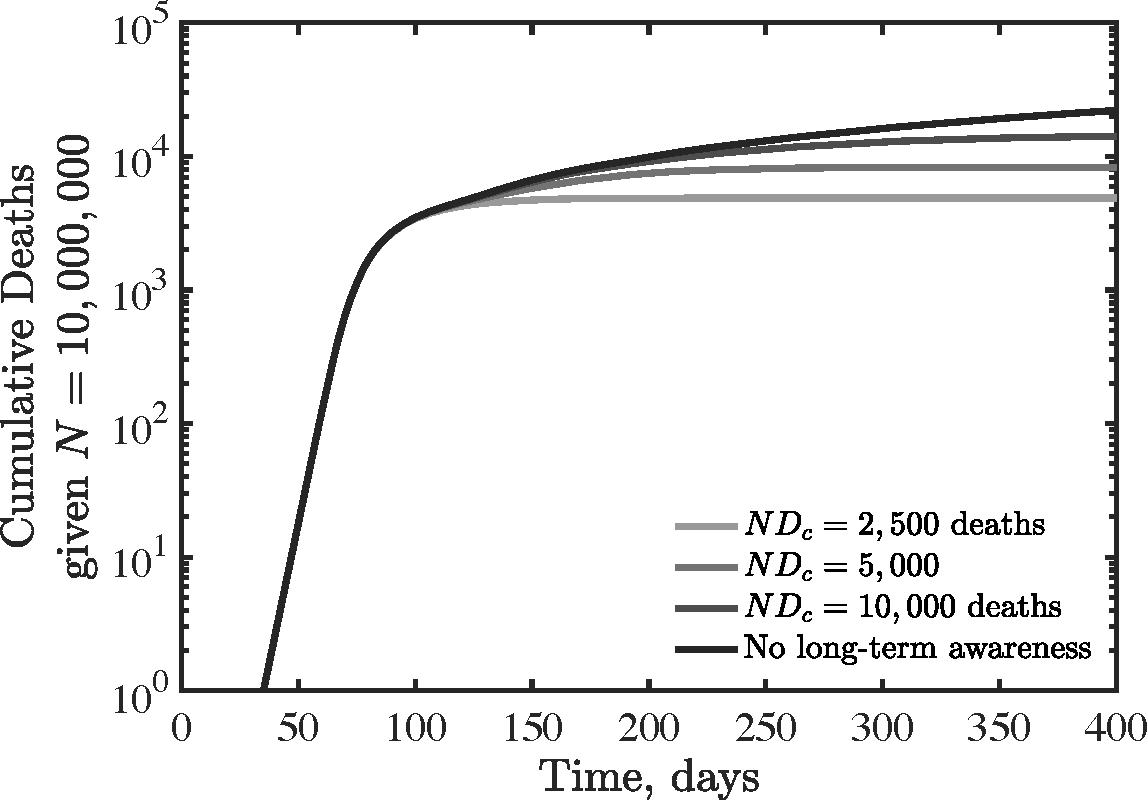
\includegraphics[width=0.47\textwidth]{scripts/figseir_Hlong_k2Dtot_noname.pdf}\\
\caption{SEIR dynamics with short- and long-term awareness.
Model parameters are $\beta=0.5$ /day, $\mu=1/2$ /day, $\gamma=1/6$ /day,
$T_H=14$ days, $f_D=0.01$, $N=10^7$, $k=2$, $N\delta_c=50$ /day (short-term
awareness), with varying $ND_c$ (long-term awareness) as shown in the legend.
The dashed line (top) denotes $\delta^{(q)}$ due to short-term
distancing alone.
\label{fig.longterm}}
\end{center}
\end{figure}

\subsection{Dynamical consequences of short-term and long-term awareness}
Awareness can vary in duration, e.g., awareness
of SARS-CoV-2 may prepare individuals to more
readily adopt and retain
social distancing measures~\citep{chen_2020social,leung_lancet2020}.  
In previous
work, long-term awareness of cumulative incidence
was shown to lead to substantial decreases
in final size of epidemics compared
to baseline expectations from inferred 
strength~\citep{eksin2019systematic}. Hence, 
we consider an extension of the SEIR model
with lags between infection and fatalities that incorporates
both short-term and long-term awareness:
\begin{eqnarray}
\dot{S} &=& -\frac{\beta SI}{\left[1+\left(\delta/\delta_c\right)^{k}+\left(D/D_c\right)^k\right]}\\
\dot{E} &=& \frac{\beta SI}{\left[1+\left(\delta/\delta_c\right)^{k}+\left(D/D_c\right)^k\right]}-\mu E\\
\dot{I} &=& \mu E-\gamma I \\
\dot{R} &=& (1-f_D)\gamma I\\
\dot{H} &=& f_D\gamma I - \gamma_H H\\
\dot{D} &=& \gamma_H H
\end{eqnarray}
where $D_c$ denotes a critical cumulative fatality level
(and formally a half-saturation constant for the impact
of long-term awareness on distancing).
Note that the relative importance of short- and long-term
awareness can be modulated by $\delta_c$ and $D_c$ respectively.
Figure~\ref{fig.longterm} shows 
daily fatalities (top)
and cumulative fatalities (bottom)
for an SEIR model with ${\cal{R}}_0=2.5$, $T_H=14$ days, and $N\delta_c=50$ 
fatalities per day and critical cumulative fatalities of
$ND_c=2,500$, 5,000, 10,000 as well as a comparison case with vanishing
long-term awareness. As is evident, 
long-term awareness drives dynamics towards rapid declines
after reaching a peak. This decline arises because
$D$ monotonically increases;
increasing fatalities beyond $D_c$ leads to rapid suppression
of transmission.  However, when $\delta_c$ rather than
$D_c$ drives dynamics, then shoulders and plateaus can re-emerge.
In reality, we expect that individual
behavior is shaped by short- and long-term awareness of risks, including
the potential for fatigue and `decay' of long-term behavior
change~\citep{funk2009spread,funk2010modelling}.

\subsection{Empirical assessment of mechanistic drivers of asymmetric peaks in Covid-19 death rates}

%Hence, we evaluated the shape of state-level epidemic peaks in the early part
%of the epidemic. In doing so, we measure the degree of asymmetry in
%the shape of empirical fatality time series.  
%To do so, we 
%find the time at which the death rate reached 10\% of its local peak
%and then compare the death rate an equivalent time period after the
%peak (see Methods).  If symmetric, these death rates should 
%be approximately equal; and note that peaks in herd-immunity
%driven SIR models have symmetry coefficients in the range of X-Y
%for ${\cal{R}}_0\approx 3$ (see Supplementary Figure X). Instead, many states 
%exhibited significantly asymetric peaks such
%that the fatality rates after peaks remained elevated.
%, i.e., sharp
%rises to the peak followed by but shallow or shoulder-like declines.
%\textbf{INSERT description of findings, reference Figure...
%For example, in Louisiana... in contrast ....}
These models suggest that 
awareness-driven distancing can drive
asymmetric epidemic peaks.
To test this hypothesis mechanistically, we jointly analyzed the dynamics of fatality
rates and behavior, using mobility
data obtained from Google COVID-19 Community Mobility Reports (https://www.google.com/covid19/mobility/)
as a proxy for behavior (see Methods for the
aggregation of multiple mobility metrics via
a Principal Component Analysis (PCA)).
Notably, we find that aggregated rates of mobility 
typically began to \emph{increase} before
the local peak in fatality was reached (Figure~\ref{fig.phase_real_theory}A).  
This rebound in mobility rates
implies that real populations are opening up faster than our simple model could predict.
%%Mobility increases while deaths increase
%is the opposite of model predictions given short- or
%long-term awareness.
Awareness-driven models, shown in Figure~\ref{fig.phase_real_theory}B,
generally show `counter-clockwise' dynamics, with risk behavior increasing up to the peak, and slowly increasing soon after.
The asymmetry here is driven by long-term awareness. 
Models with short-term awareness but no long-term awareness exhibit a tight link between fatality and behavior (``reversible'' behavior, like the top curve in  Figure~\ref{fig.phase_real_theory}B. 

In contrast, the real data (Figure~\ref{fig.phase_real_theory}A) show mostly clockwise dynamics, with NY state a nearly reversible (but still clockwise) pattern, and only Washington state showing the counter-clockwise pattern predicted by the simple model.
%Given short-term awareness,
%individuals distance as deaths increase (reducing mobility), driving down
%deaths, which leads to an increase in mobility, albeit along
%the same curve in the phase plane (similar to the NY state trajectory).
%Yet, with long-term awareness, then given sufficient deaths, behavior
%is driven down and remains low, as individual behavior is shaped
%by the cumulative deaths (unlike any observed trajectory). 
We hypothesized that
a combination of awareness-driven distancing and fatigue
could lead to clockwise dynamics: if people become fatigued with distancing behavior, then risk could rise even as deaths were rising.
We developed the following model as a proof of concept in which
the fatigue is driven directly by deaths (though alternatives
could also be explored linked to cases, hospitalizations, deaths 
and/or a combination):
\begin{eqnarray}
\dot{S} &=& -\beta g(D) SI\\
\dot{E} &=& beta g(D) SI-\mu E\\
\dot{I} &=& \mu E-\gamma I \\
\dot{R} &=& (1-f_D)\gamma I\\
\dot{H} &=& f_D\gamma I - \gamma_H H\\
\dot{D} &=& \gamma_H H \\
\dot{\beta} &=&\frac{\epsilon}{2}\left[\frac{\left(\frac{\hat{\beta}}{1+\left(\delta/\delta_c\right)^{k}}-\beta\right)}{1+\left(D/D_c\right)^k}+\left(\hat{\beta}-\beta\right)\right] \label{eq.fatigue}
\end{eqnarray}


\begin{figure*}
\begin{center}
\mbox{\hspace{0.05\textwidth}}
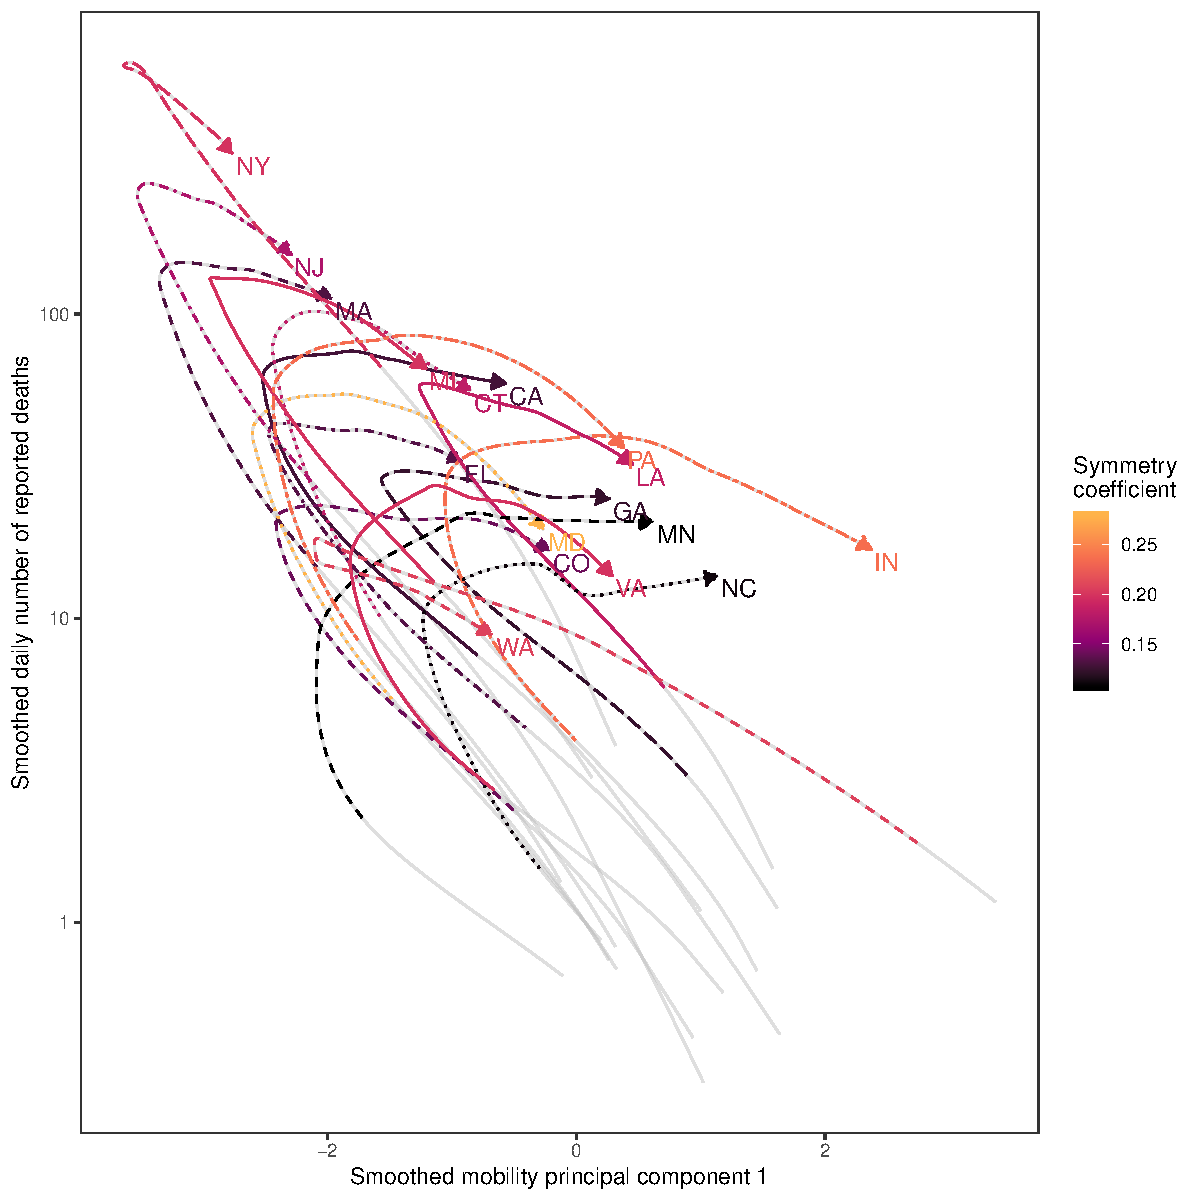
\includegraphics[width=0.5\textwidth]{deaths/national_deaths_metric_phase_pca_grand.pdf}\\
\includegraphics[width=0.325\textwidth]{scripts/figseir_phase2_noname.pdf}
\includegraphics[width=0.325\textwidth]{scripts/figseir_phase2_statefix_noname.pdf}
\includegraphics[width=0.325\textwidth]{scripts/figseir_phase2_state_noname.pdf}
\caption{Phase-plane visualizations of deaths vs.~mobility for state-level
data (top) and SEIR models (bottom panels).
(Top) Deaths and mobility indexes through time for the 17 analyzed states. Both data series are smoothed. 
Time windows as in \ref{fig.plateaus_cases}.
(B)
Dynamics of effective behavior and death rates
in a SEIR model with short- and long-term awareness. 
Curves denote different assumptions regarding long-term awareness,
in each case $\beta=0.5$/day, $\mu=0.5$/day, $\gamma=1/6$/day, such that ${\cal{R}}_0=3$,
with $k=2$, $\gamma_H=1/21$/day, and $f_D=0.01$.  The short-term awareness
corresponds go $N\delta_c=50$ deaths/day. Thin lines denote
full dynamics over 400 days; thick lines denote the dynamics
near the case fatality peak.
(C) Dynamics of effective behavior and death rates
in a SEIR model with awareness and fatigue. The three
different curves denote different assumptions regarding long-term awareness,
in each case $\beta=0.5$/day, $\mu=0.5$/day, $\gamma=1/6$/day, such that ${\cal{R}}_0=3$,
with $k=2$, $\gamma_H=1/21$/day, $f_D=0.01$, and $\epsilon=1/7$/day.  
The short-term awareness
corresponds go $N\delta_c=50$ deaths/day. 
The force of infection does not include long term changes in behavior
beyond mobility, i.e., $g(D)=1$.
(D) As in (C), but the force
of infection includes long-term changes in behavior, i.e., 
$g(D)=1/\left(1+(D/D_c)^k\right)$.
\label{fig.phase_real_theory}}
\end{center}
\end{figure*}


In this model with fatigue,
the force of infection is related to the
mobility denoted by $\beta(t)$ (which dictates
the number of interactions per unit time) modulated by
a reduction in risk per infection $g(D)$.
In this model,
$\hat{\beta}$ denotes the baseline behavior,
and $\epsilon$ denotes a time-scale for behavior change.  
%Note
%that in the limit of $\delta=0$ and $D=0$, then $\beta$
%asymptotically approaches $\hat{\beta}$ given a time scale $1/\epsilon$
%in the absence of fatalities. 
The level of fatigue is controlled by $D_c$, such that
mobility returns to a baseline $\hat{\beta}$ once $D\gg D_c$.
We consider two models, corresponding to
$g(D)=1$ such that the force of infection depends on mobility alone,
and 
$g(D)=1/\left(1+(D/D_c)^k\right)$
corresponding to sustained changes in the risk of infection
per contact (e.g., due to mask wearing, contact-less
interactions, use of PPE, etc.). 
As shown in Figure~\ref{fig.phase_real_theory}C/D, the dynamics 
switch from counter-clockwise to clockwise in the $\delta-\beta$ plane
given the incorporation of fatigue.
Deaths drive down mobility, but eventually,
decreases in $\beta$ due to short-term awareness
are over-come by fatigue, leading to increases in $\beta$.
If $g(D)=1$, then 
the dynamics include increases in both mobility and fatalities
akin to levels expected in the absence of behavior, and eventually
levels of infection that are stopped by herd immunity, rather than by 
awareness (see Figure~\ref{fig.phase_real_theory}C).  
In contrast, if there is sustained behavior change
such that $g(D)$ increases with increasing cumulative deaths
then there is a single peak that forms a clockwise loop; with
the peak close to, but after the minimum in behavior (Figure~\ref{fig.phase_real_theory}D); as observed in nearly all state-level data sets.
%This analysis reveals a complex interplay between short-term awareness,
%long-term awareness, and fatigue, can generate qualitative
%signatures consistent with empirical observations.

\section{Conclusions}
We have developed and analyzed
a series of models that assume awareness of disease-induced death can 
reduce transmission and shown that such awareness-driven feedback
can lead
to highly asymmetric epidemic curves.  Asymmetric
curves exhibit extended periods of near-constant
cases even as the majority of the population remains susceptible.
Hence: passing a `peak' need not imply
the rapid decline of risk.  
In these conditions, if individuals are unable
to sustain social
distancing policies, or begin to tolerate higher death rates, then cases 
could increase (similar results have also been proposed in a recent, independently derived feedback SIR model~\citep{franco2020feedback}). 
Indeed, detailed analysis of mobility and fatalities suggest
that mobility increased before fatalities peak.
This is not consistent with simple models of awareness-driven distancing, but is consistent with more detailed models.
We show that decay of distancing behavior due to fatigue can produce dynamics of this sort; other mechanisms are also possible.
\jd{This s. reads like a tautology.} Notably we find that if mobility increases but the risk of infection per interaction decreases due to systemic changes in behavior, then models suggest `clockwise' dynamics between behavior and fatality as found in nearly all state-level data sets analyzed here.
Awareness-driven endogenous changes in ${\cal{R}}_{\mathrm{eff}}$ are typically
absent in models that form the basis for public policy and strategic planning.
Our findings highlight the potential impacts of short-term and long-term awareness in efforts to shape information campaigns to reduce transmission after early onset `peaks', particularly when populations remain predominantly immunologically naive.

Although the models here are intentionally simple,
it seems likely that observed asymmetric dynamics of COVID-19, including
slow declines and plateau-like behavior, is an emergent
property of awareness-driven epidemiological dynamics.
%
%We recognize that qualititatively similar effects could arise 
%if responses are due to case reports or to illnesses
%with a personal connection. They may also be driven by official and media responses, as well as purely individual ones. In addition, ongoing ascertainment
%biases may also influence the shape of reported, rather
%than actual, case curves.  
%
Moving forward, it is essential to fill in significant
gaps in understanding how awareness of disease
risk and severity shape behavior~\citep{west_nat2020}. 
Mobility data is a proxy but
not equivalent to a direct indicator of transmission
risk. Thus far, measurements of community
mobility have been
used as a leading indicator for epidemic outcomes.
Prior work has shown significant impacts of changes
in mobility and behavior on the COVID-19 outbreak~\citep{kraemer_2020sci}.
Here we have
shown the importance of looking at a complementary feedback
mechanism,
i.e., from outbreak to behavior.  
In doing so, we have also shown that decomposing the 
force of infection in terms of the number of potential
transmissions and the probability of infection per contact
can lead to outcomes aligned with observed state-level dynamics.
%This feedback is key given
%that many mobility studies suggested that individuals began
%social distancing before shelter-in-place policies were instituted.
Understanding the drivers behind emergent plateaus observed
at national and sub-national levels could help decision
makers structure intervention efforts appropriately to effectively 
communicate awareness campaigns that may aid in collective
efforts to control the ongoing COVID-19 pandemic.

\section{Methods}

\subsection{Epidemiological data}

Daily number of reported deaths as of June 7, 2020, is obtained from The COVID Tracking Project (covidtracking.com).

\subsection{Mobility data}

Mobility data as of June 12, 2020, are obtained from Google COVID-19 Community Mobility Reports (www.google.com/covid19/mobility/).
The data set describes percent changes in mobility across six categories (grocery and pharmacy; parks; residential; retail and recreation; transit; and workplaces)
compared to the median value from the 5--week period Jan 3--Feb 6, 2020.
Raw mobility data are plotted in Supplementary Figure~\ref{fig.supp_mobility}.

\subsection{Principal component analysis}

We use principal component analysis (PCA) on the mobility data to obtain a univariate index of mobility. 
We exclude park visits from the analysis due to their anomalous, noisy patterns (Supplementary Figure~\ref{fig.supp_mobility}).
Before performing PCA, we first calculate the 7-day rolling average for each mobility measure in order to remove the effects of weekly patterns.
We combined mobility data from all 17 analyzed states, and standardized each measure (to zero mean and unit variance). 
The first principal component explains 93\% of the total variance in this analysis, and the loading of the residential metric had a different sign from the other four mobility metrics. 
We thus used this component as our index of mobility (setting the direction so that only the residential metric contributed negatively to the index).
To draw phase planes, we further smoothed our mobility index and daily reported deaths using locally estimated scatterplot (LOESS) smoothing.
Daily number of deaths is smoothed in log space, only including days with one or more reported deaths.
LOESS smoothing is performed by using the \texttt{loess} function in \texttt{R}.

%\begin{figure}
%\begin{center}
%\includegraphics[width=0.45\textwidth]{figseir_phase2_noname.pdf}
%\caption{Dynamics of effective behavior and death rates
%in a SEIR model with short- and long-term awareness. The four
%curves denote different assumptions regarding long-term awareness,
%in each case $\beta=0.5$, $\mu=0.5$, $\gamma=1/6$, such that ${\cal{R}}_0=3$,
%with $k=2$, $\gamma_H=1/21$, and $f_D=0.01$.  The short-term awareness
%corresponds go $N\delta_c=50$ deaths/day. Thin lines denote
%full dynamics over 400 days; thick lines denote the dynamics
%near the case fatality peak.
%\label{fig.phase_theory}}
%\end{center}
%\end{figure}

%\begin{figure*}
%\begin{center}
%\includegraphics[width=0.45\textwidth]{figseir_phase2_state_noname.pdf}
%\mbox{\hspace{0.05\textwidth}}
%\includegraphics[width=0.45\textwidth]{figseir_phase2_statefix_noname.pdf}
%\caption{
%Dynamics of effective behavior and death rates
%in a SEIR model with awareness and fatigue. The three
%different curves denote different assumptions regarding long-term awareness,
%in each case $\beta=0.5$, $\mu=0.5$, $\gamma=1/6$, such that ${\cal{R}}_0=3$,
%with $k=2$, $\gamma_H=1/21$, $f_D=0.01$, and $\epsilon=1/7$.  
%The short-term awareness
%corresponds go $N\delta_c=50$ deaths/day. (A) The force
%of infection includes long-term changes in behavior, i.e., $\beta SI/\left(1+(D/D_c)^k\right)$.
%(B) The force of infection does not include long term changes in behavior
%beyond mobility, i.e., $\beta S I$.
%\label{fig.phase_fatigue}}
%\end{center}
%\end{figure*}
